\chapter{Manual de usuario}

\section{Perfil de usuario}
\addtocounter{figura_manual}{1} Para comenzar, tenemos la página de inicio de la web (\textbf{\hyperref[fig:Web_Index_Usuario]{Figura 6.\arabic{figura_manual}}}). Desde ella podremos acceder a las distintas funciones disponibles dependiendo del perfil con el que se haya accedido.
\begin{figure}[!htbp]
  \centering
  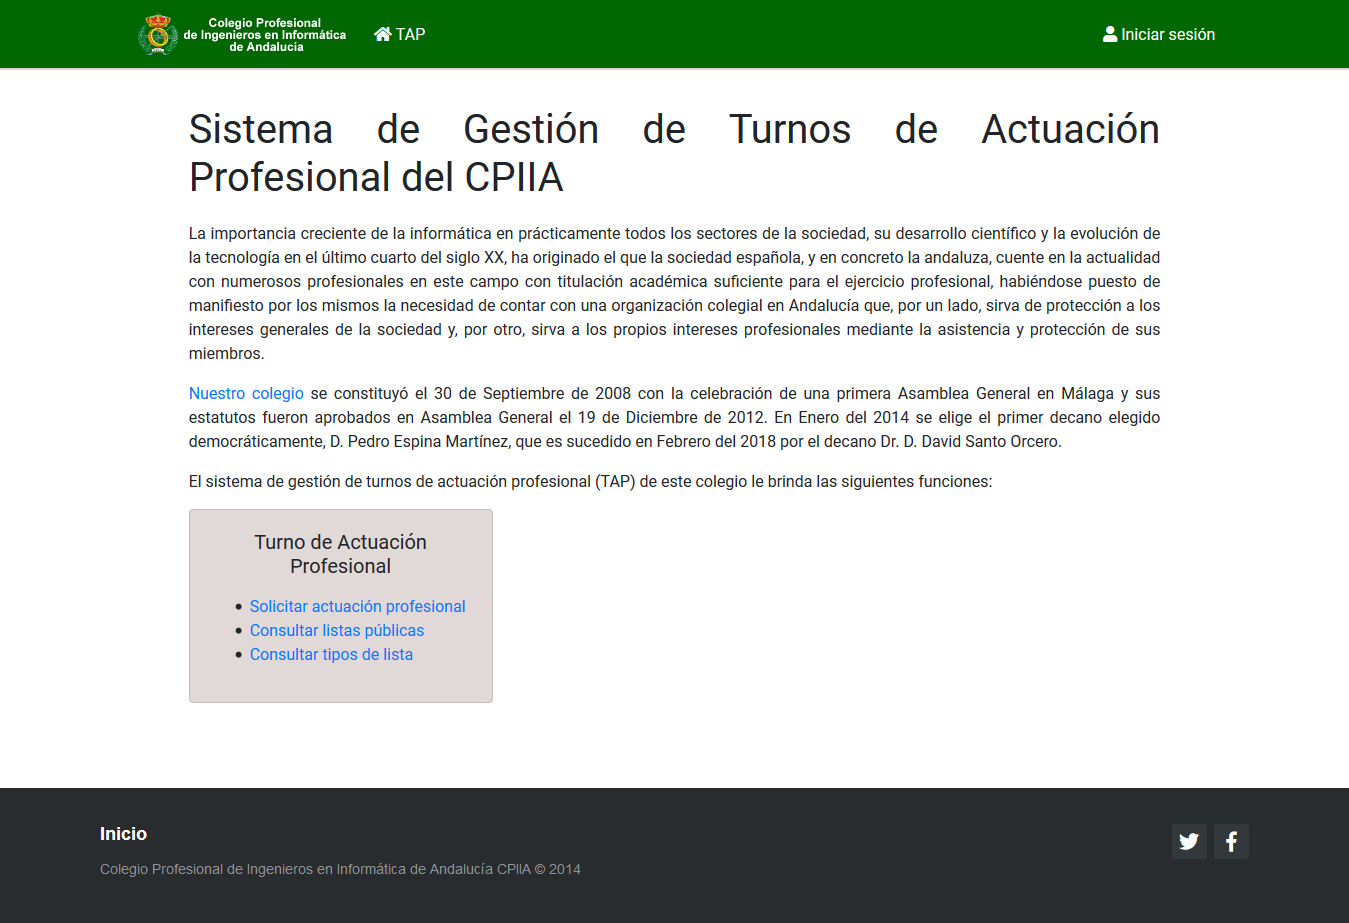
\includegraphics[width=150mm]{Web/Index_Usuario.png}
  \caption{Página de Inicio (Usuario)}
  \label{fig:Web_Index_Usuario}
\end{figure}
\FloatBarrier

\addtocounter{figura_manual}{1} Como Usuario, solo se tendrá acceso a la solicitud de actuación profesional y a la consulta de listas públicas y tipos de lista. Para la solicitar la actuación de un profesional deberá rellenar los campos mostrados en la \textbf{\hyperref[fig:Web_TAP_SolicitarActuacion]{Figura 6.\arabic{figura_manual}}} y pulsar el botón ``Enviar Solicitud''.
\begin{figure}[!htbp]
  \centering
  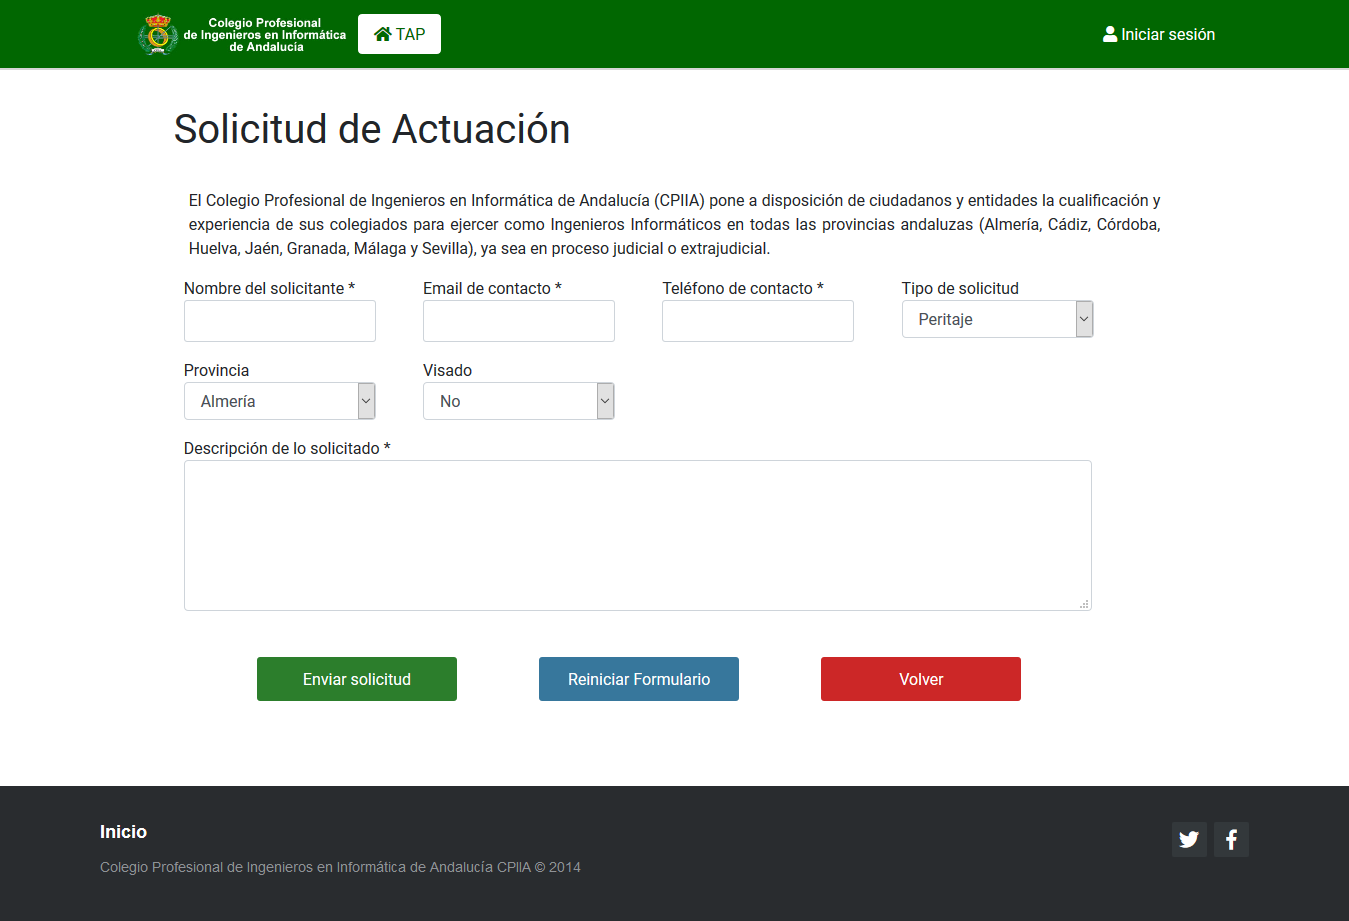
\includegraphics[width=150mm]{Web/TAP_SolicitarActuacion.png}
  \caption{Solicitud de Actuación de un Profesional (Usuario)}
  \label{fig:Web_TAP_SolicitarActuacion}
\end{figure}
\FloatBarrier

\addtocounter{figura_manual}{1} Para el caso de consultar los colegiados inscritos en las listas públicas, tendremos que seleccionar el tipo de lista y el territorio y pulsar el botón ``Buscar''. Tras esto, aparecerá el listado de colegiados inscritos en la lista pública en cuestión (\textbf{\hyperref[fig:Web_TAP_ListasPublicas]{Figura 6.\arabic{figura_manual}}}).
\begin{figure}[!htbp]
  \centering
  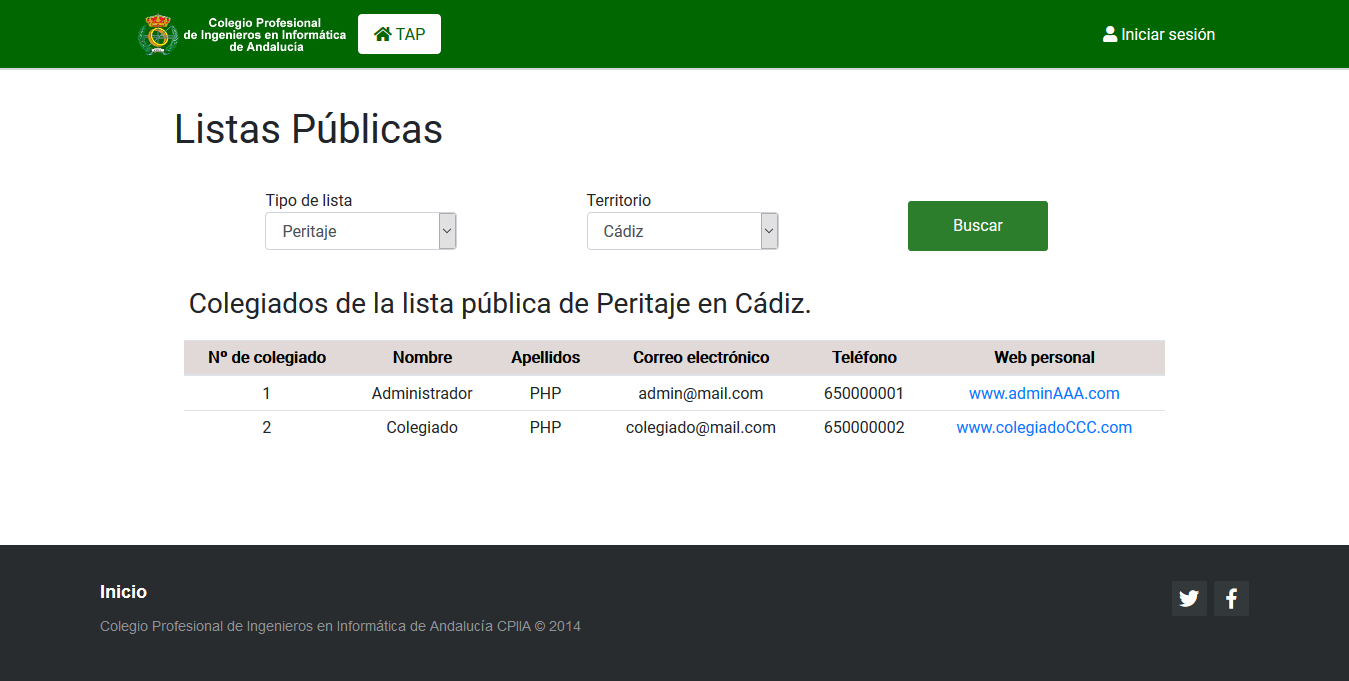
\includegraphics[width=150mm]{Web/TAP_ListasPublicas.png}
  \caption{Listas Públicas (Usuario)}
  \label{fig:Web_TAP_ListasPublicas}
\end{figure}
\FloatBarrier

\addtocounter{figura_manual}{1} Y en la consulta de tipos de lista únicamente se muestran los mismos y la descripción de cada uno (\textbf{\hyperref[fig:Web_TAP_TiposLista]{Figura 6.\arabic{figura_manual}}}).
\begin{figure}[!htbp]
  \centering
  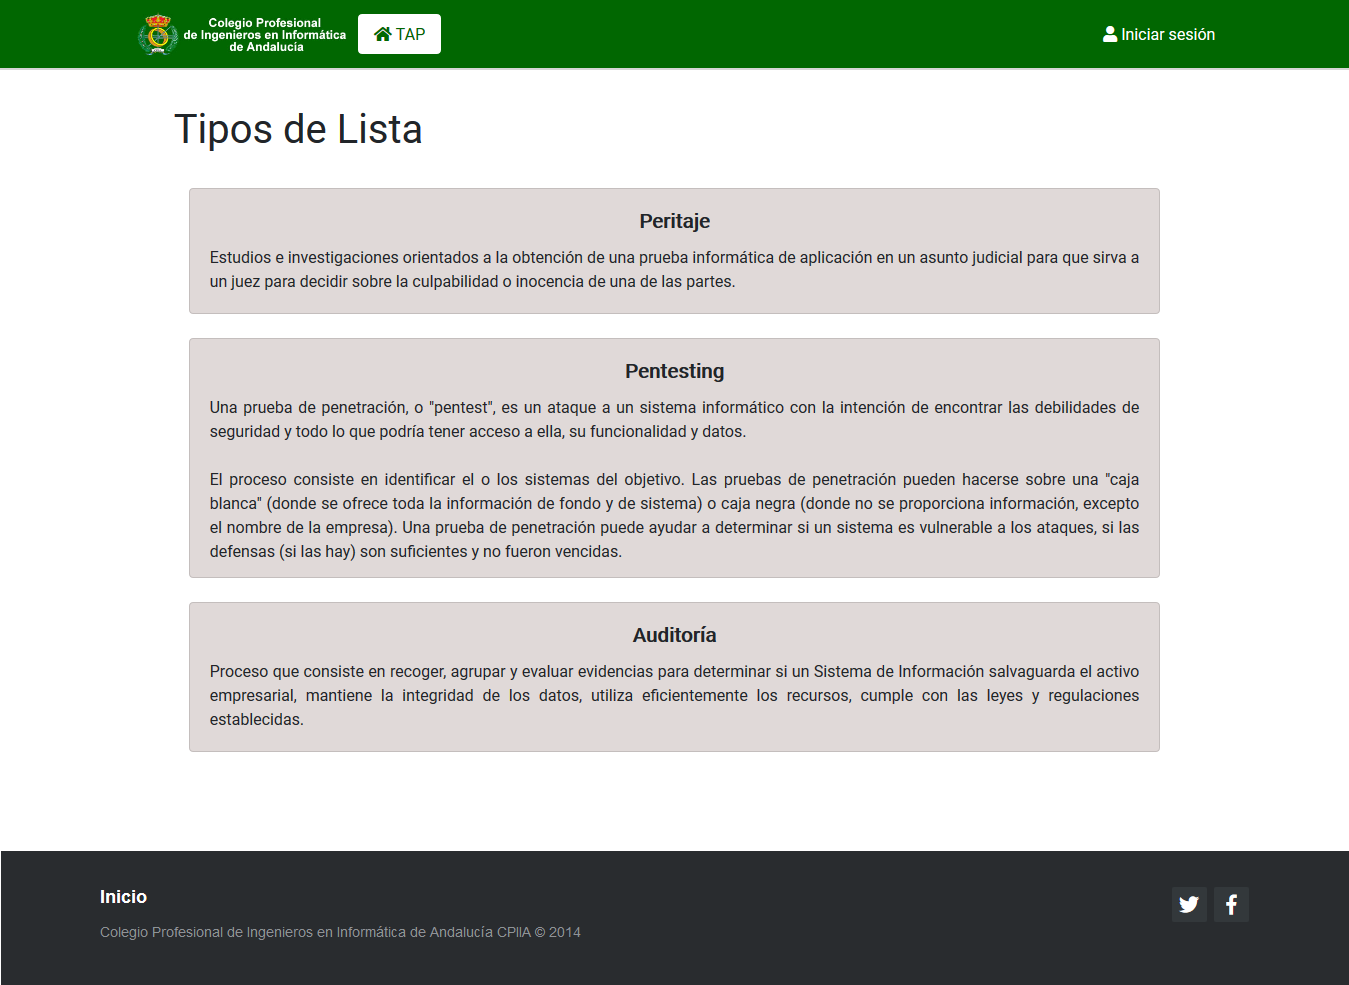
\includegraphics[width=150mm]{Web/TAP_TiposLista.png}
  \caption{Tipos de Lista (Usuario)}
  \label{fig:Web_TAP_TiposLista}
\end{figure}
\FloatBarrier


\section{Perfil de colegiado}
\addtocounter{figura_manual}{1} Teniendo un número de colegiado asignado, ya será posible identificarse ante el sistema. Para ello hay que acceder a la vista de ``Iniciar Sesión'' (\textbf{\hyperref[fig:Web_Login]{Figura 6.\arabic{figura_manual}}}).\addtocounter{figura_manual}{1} Una vez introducidos el número de colegiado y la contraseña habrá que pulsar el botón ``Entrar'' y si ambos son correctos se le reenviará a la página de inicio, ya identificado como colegiado (\textbf{\hyperref[fig:Web_Index_Colegiado]{Figura 6.\arabic{figura_manual}}}).
\begin{figure}[!htbp]
  \centering
  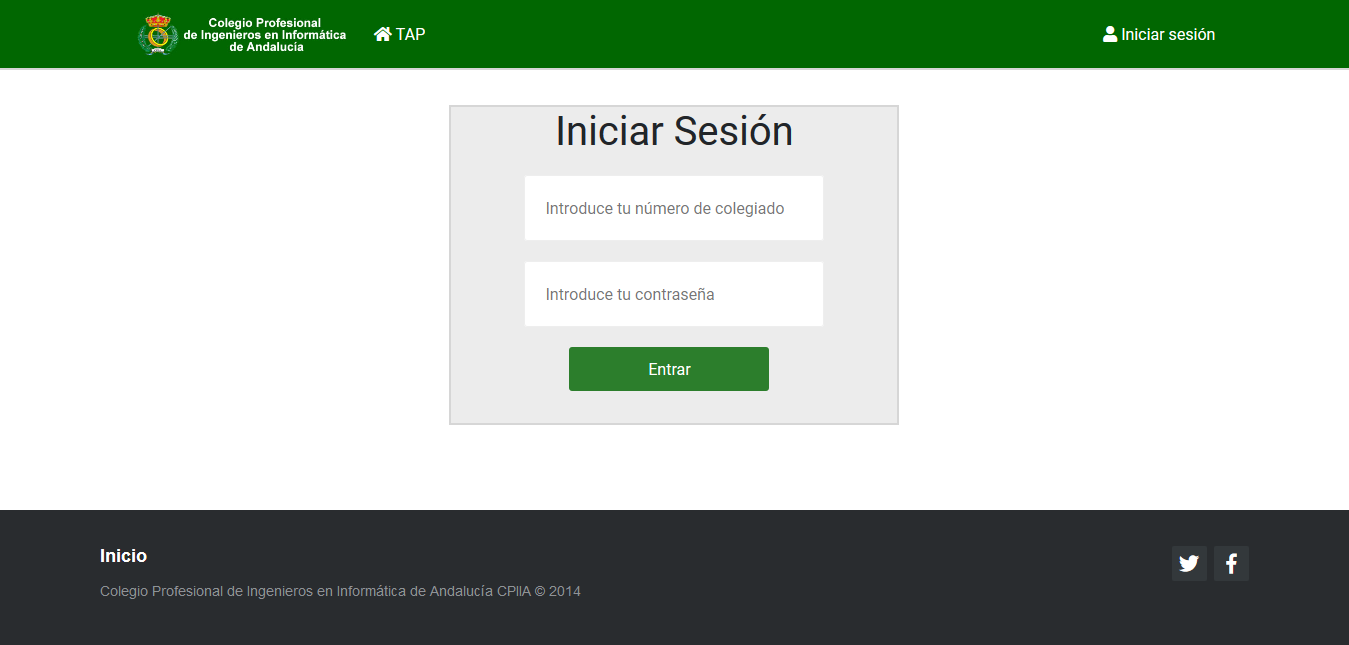
\includegraphics[width=150mm]{Web/Login.png}
  \caption{Iniciar Sesión}
  \label{fig:Web_Login}
\end{figure}
\FloatBarrier

\begin{figure}[!htbp]
  \centering
  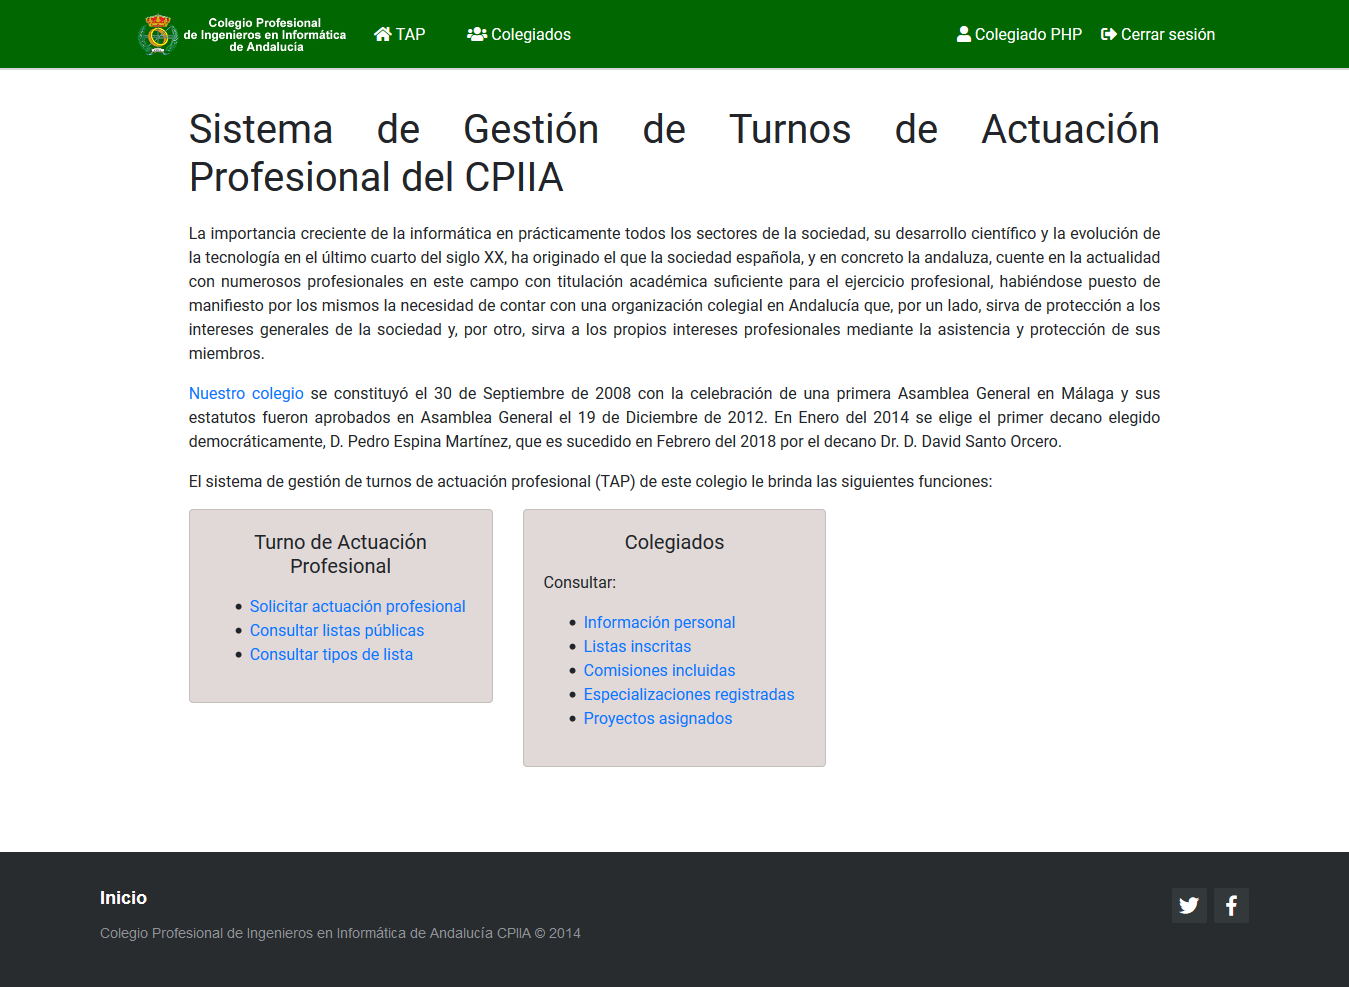
\includegraphics[width=150mm]{Web/Index_Colegiado.png}
  \caption{Página de Inicio (Colegiado)}
  \label{fig:Web_Index_Colegiado}
\end{figure}
\FloatBarrier

Una vez identificado como colegiado, tendrá la posibilidad de:
\begin{itemize}
  \item \addtocounter{figura_manual}{1} Consultar su información personal y actualizar su contraseña desde la vista ``Mi Perfil'' (\textbf{\hyperref[fig:Web_Coleg_MiPerfil]{Figura 6.\arabic{figura_manual}}}).
  \item \addtocounter{figura_manual}{1} Consultar las listas en las que esté inscrito y el número de colegiados que le preceden en ella en ``Mis Listas'' (\textbf{\hyperref[fig:Web_Coleg_MisListas]{Figura 6.\arabic{figura_manual}}}).
  \item \addtocounter{figura_manual}{1} Consultar las comisiones en las que está inscrito y el cargo que ostenta sobre ellas en ``Mis Comisiones'' (\textbf{\hyperref[fig:Web_Coleg_MisComisiones]{Figura 6.\arabic{figura_manual}}}).
  \item \addtocounter{figura_manual}{1} Consultar las especializaciones que le han sido registradas desde ``Mis Especializaciones'' (\textbf{\hyperref[fig:Web_Coleg_MisEspecializaciones]{Figura 6.\arabic{figura_manual}}}).
  \item \addtocounter{figura_manual}{1} Consultar los proyectos que le han sido asignados, su función en ellos y el estado actual del mismo desde la vista ``Mis Proyectos'' (\textbf{\hyperref[fig:Web_Coleg_MisProyectos]{Figura 6.\arabic{figura_manual}}}).
\end{itemize}

\begin{figure}[!htbp]
  \centering
  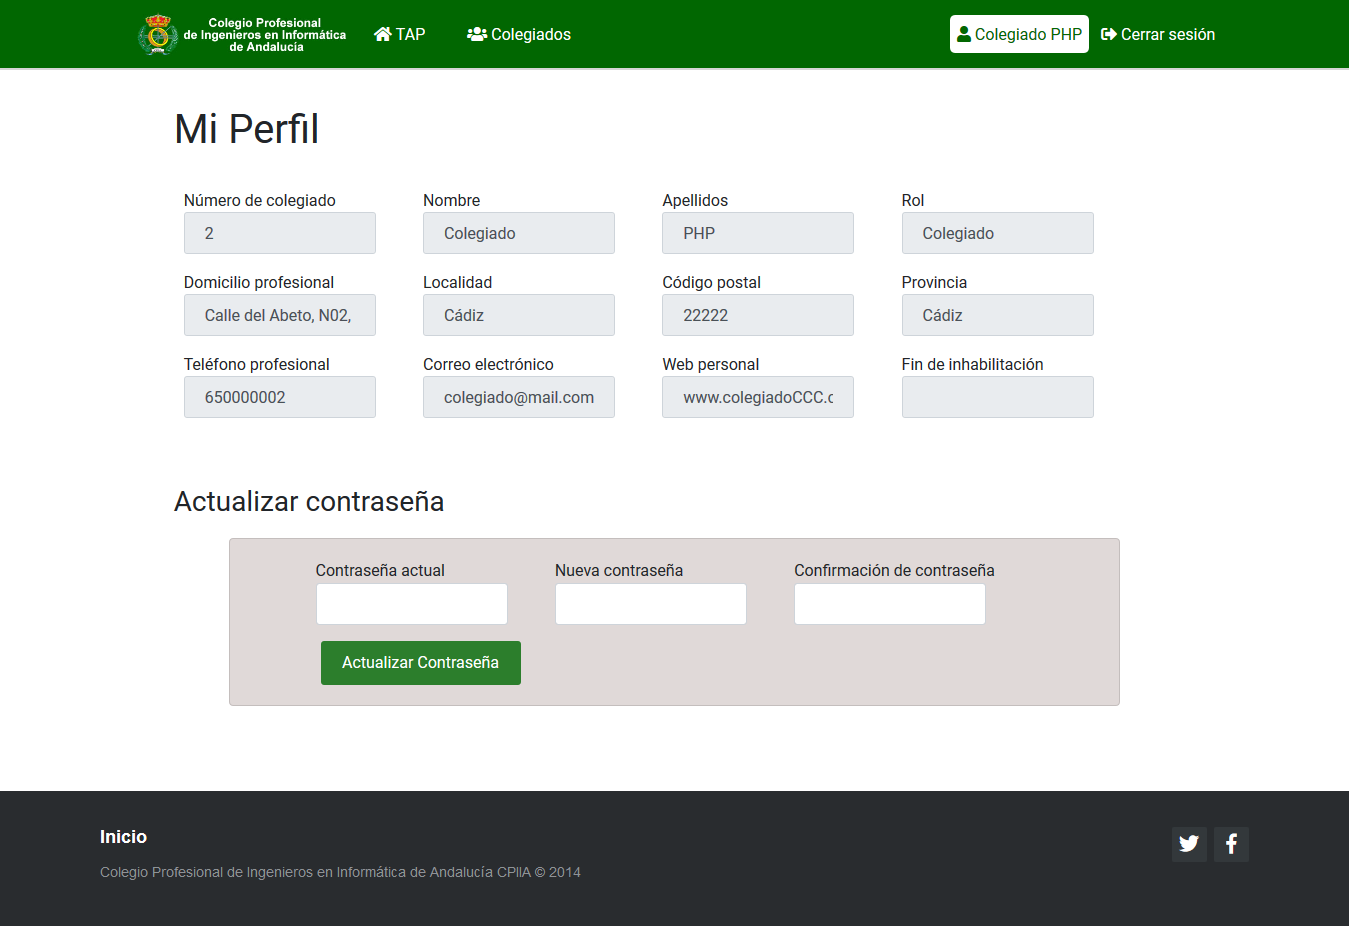
\includegraphics[width=150mm]{Web/Coleg_MiPerfil.png}
  \caption{Mi Perfil}
  \label{fig:Web_Coleg_MiPerfil}
\end{figure}
\FloatBarrier

\begin{figure}[!htbp]
  \centering
  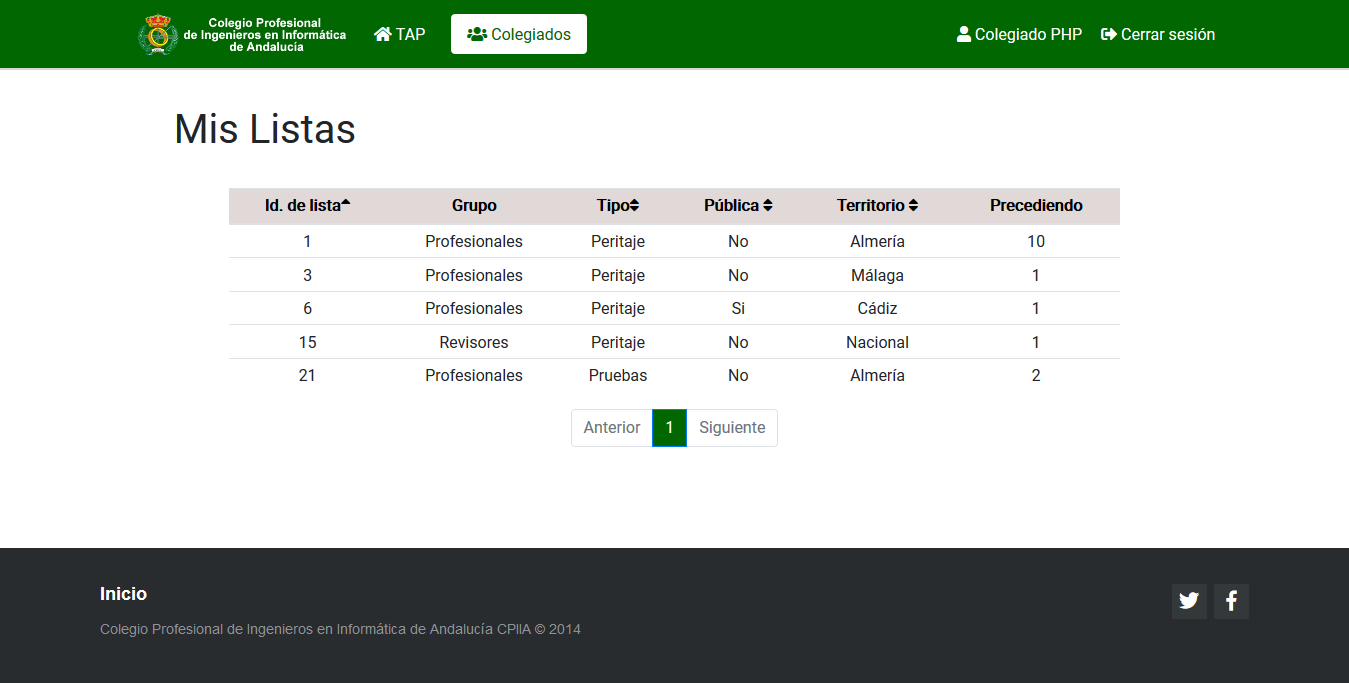
\includegraphics[width=150mm]{Web/Coleg_MisListas.png}
  \caption{Mis Listas}
  \label{fig:Web_Coleg_MisListas}
\end{figure}
\FloatBarrier

\begin{figure}[!htbp]
  \centering
  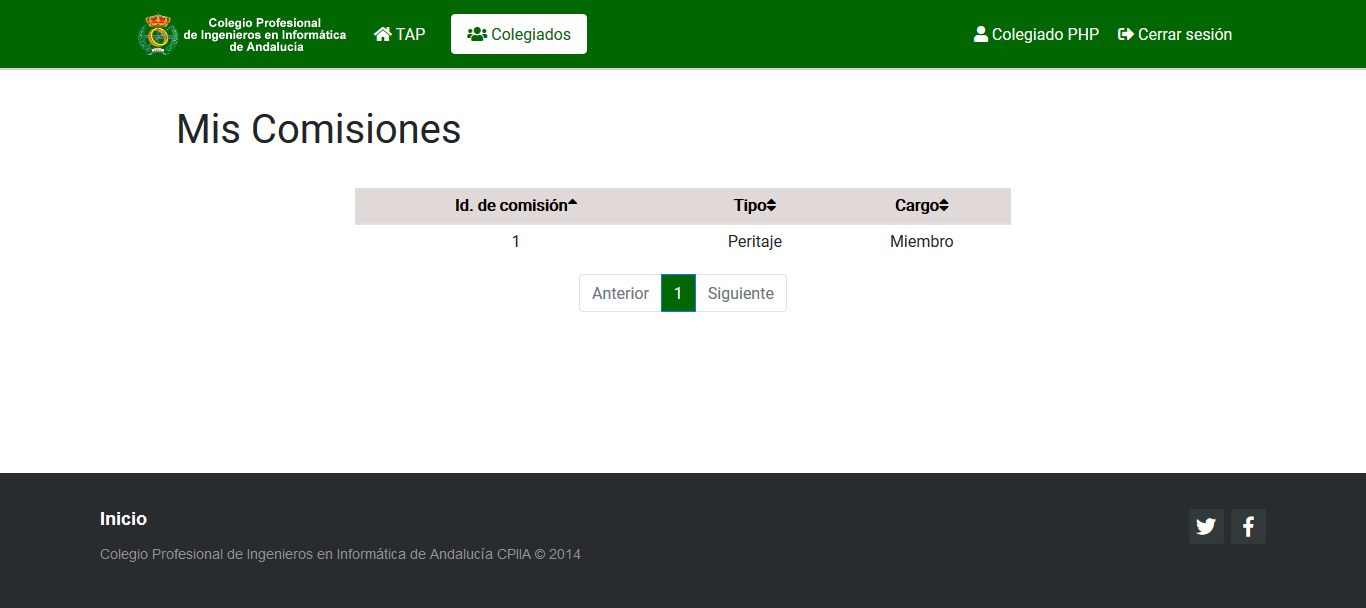
\includegraphics[width=150mm]{Web/Coleg_MisComisiones.png}
  \caption{Mis Comisiones}
  \label{fig:Web_Coleg_MisComisiones}
\end{figure}
\FloatBarrier

\begin{figure}[!htbp]
  \centering
  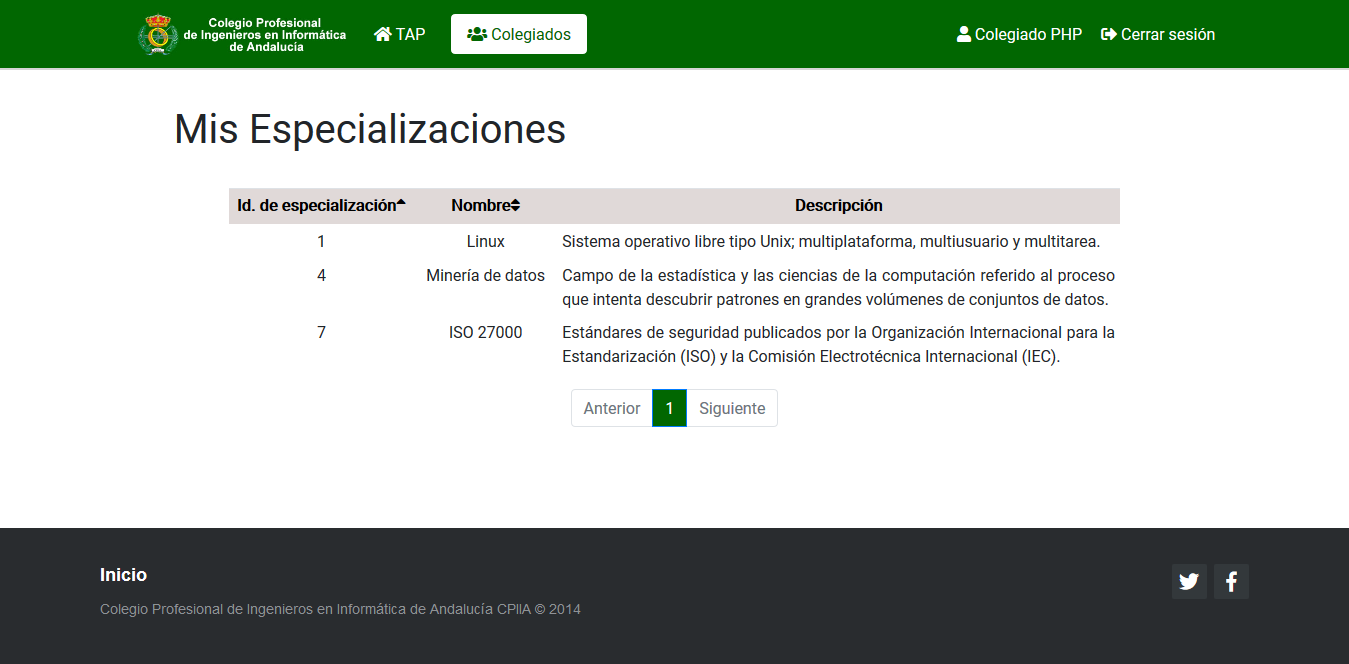
\includegraphics[width=150mm]{Web/Coleg_MisEspecializaciones.png}
  \caption{Mis Especializaciones}
  \label{fig:Web_Coleg_MisEspecializaciones}
\end{figure}
\FloatBarrier

\begin{figure}[!htbp]
  \centering
  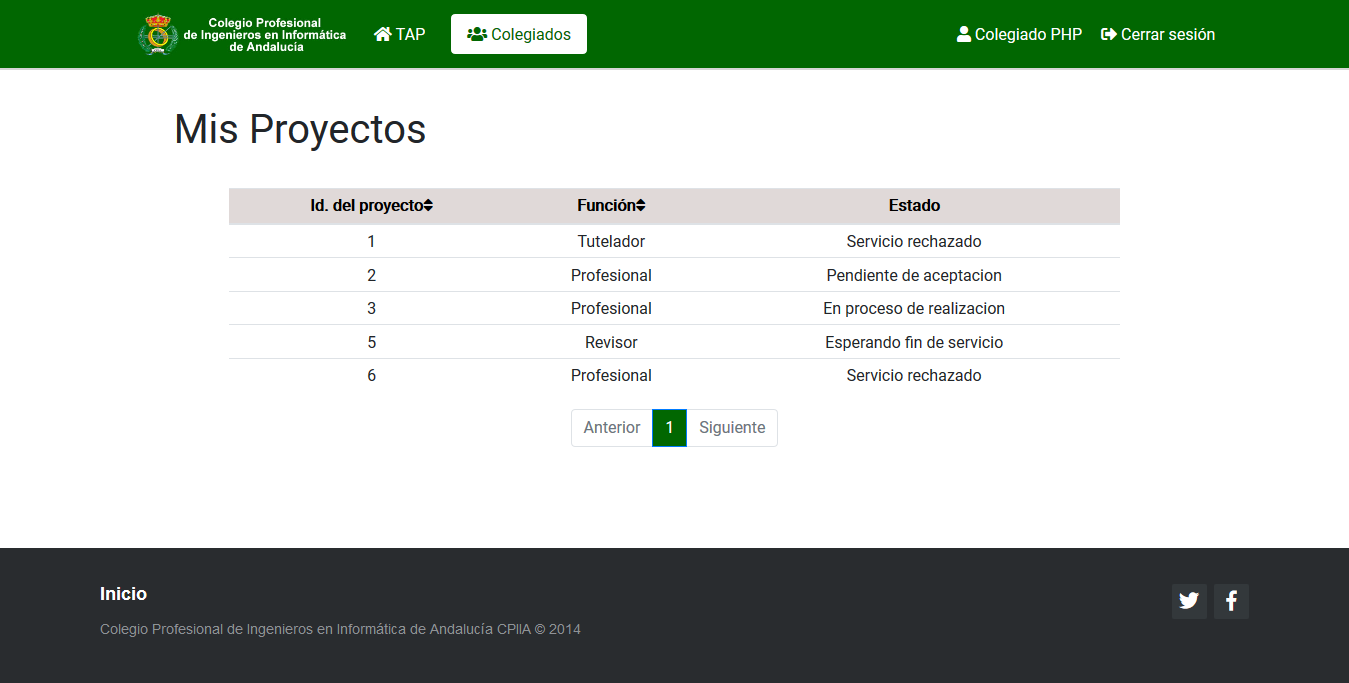
\includegraphics[width=150mm]{Web/Coleg_MisProyectos.png}
  \caption{Mis Proyectos}
  \label{fig:Web_Coleg_MisProyectos}
\end{figure}
\FloatBarrier
\newpage~


\section{Perfil de responsable}
\addtocounter{figura_manual}{1} De la misma forma que ocurre al identificarse en el sistema como colegiado, al hacerlo como responsable la interfaz de la página de inicio varía, añadiendo los enlaces a las vistas de administración de la página (\textbf{\hyperref[fig:Web_Index_Responsable]{Figura 6.\arabic{figura_manual}}}).

\begin{figure}[!htbp]
  \centering
  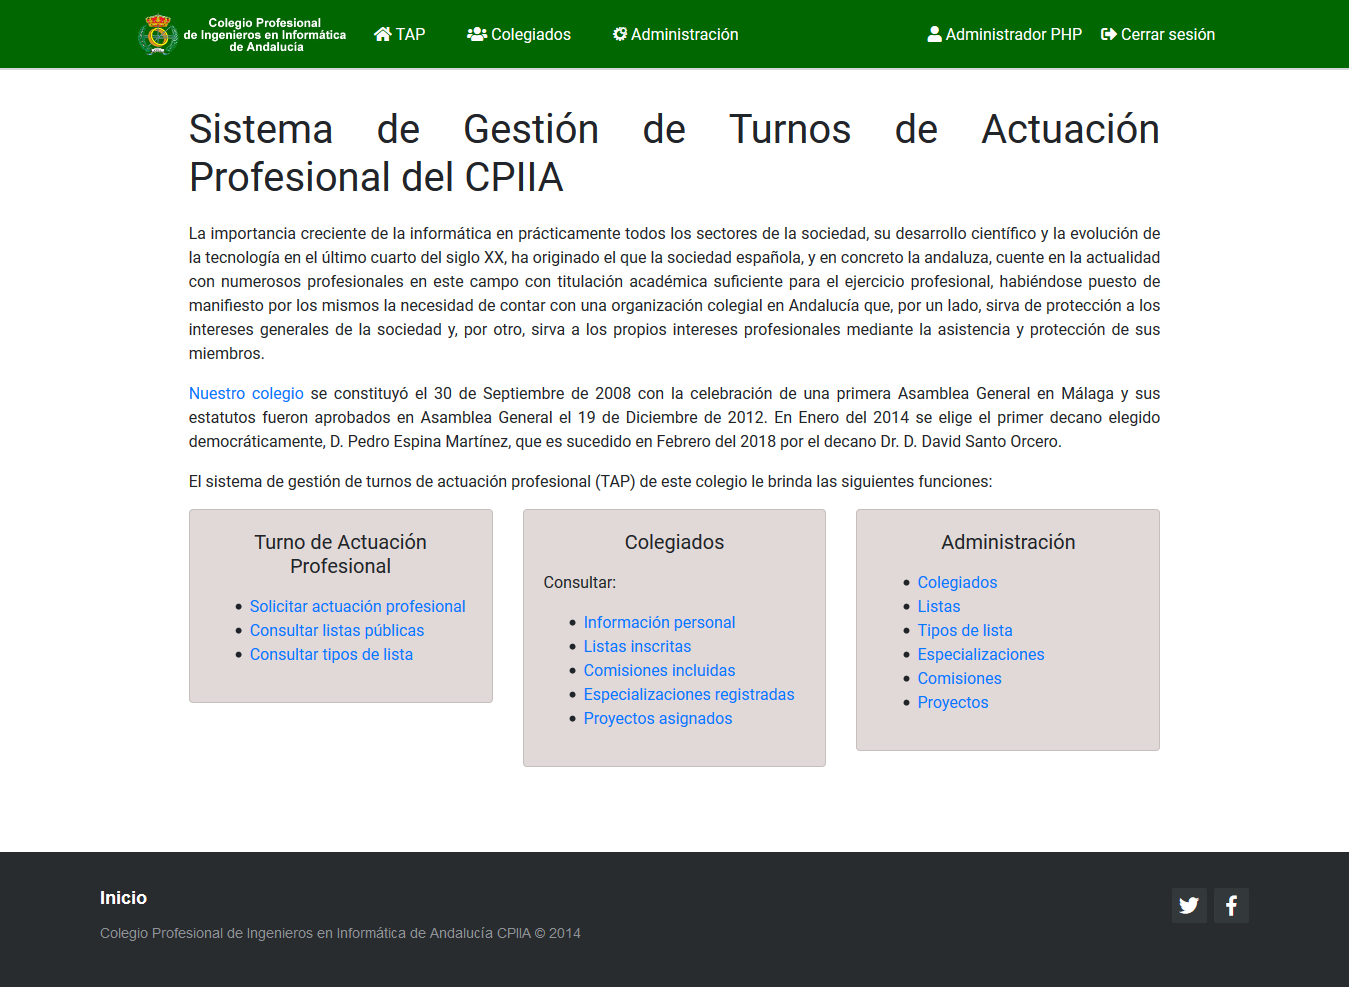
\includegraphics[width=150mm]{Web/Index_Responsable.png}
  \caption{Página de Inicio (Responsable)}
  \label{fig:Web_Index_Responsable}
\end{figure}
\FloatBarrier

\addtocounter{figura_manual}{1} En la administración de colegiados se nos muestra el conjunto de colegiados existentes en el sistema (\textbf{\hyperref[fig:Web_Admin_Colegiados]{Figura 6.\arabic{figura_manual}}}).\addtocounter{figura_manual}{1}  Desde esta vista podremos acceder a la creación de nuevos colegiados (\textbf{\hyperref[fig:Web_Admin_ColegiadoCrear]{Figura 6.\arabic{figura_manual}}}) \addtocounter{figura_manual}{1} y la consulta (\textbf{\hyperref[fig:Web_Admin_ColegiadoConsultar]{Figura 6.\arabic{figura_manual}}})\addtocounter{figura_manual}{1}  o modificación (\textbf{\hyperref[fig:Web_Admin_ColegiadoModificar]{Figura 6.\arabic{figura_manual}}}) de los ya registrados en el sistema.
\begin{figure}[!htbp]
  \centering
  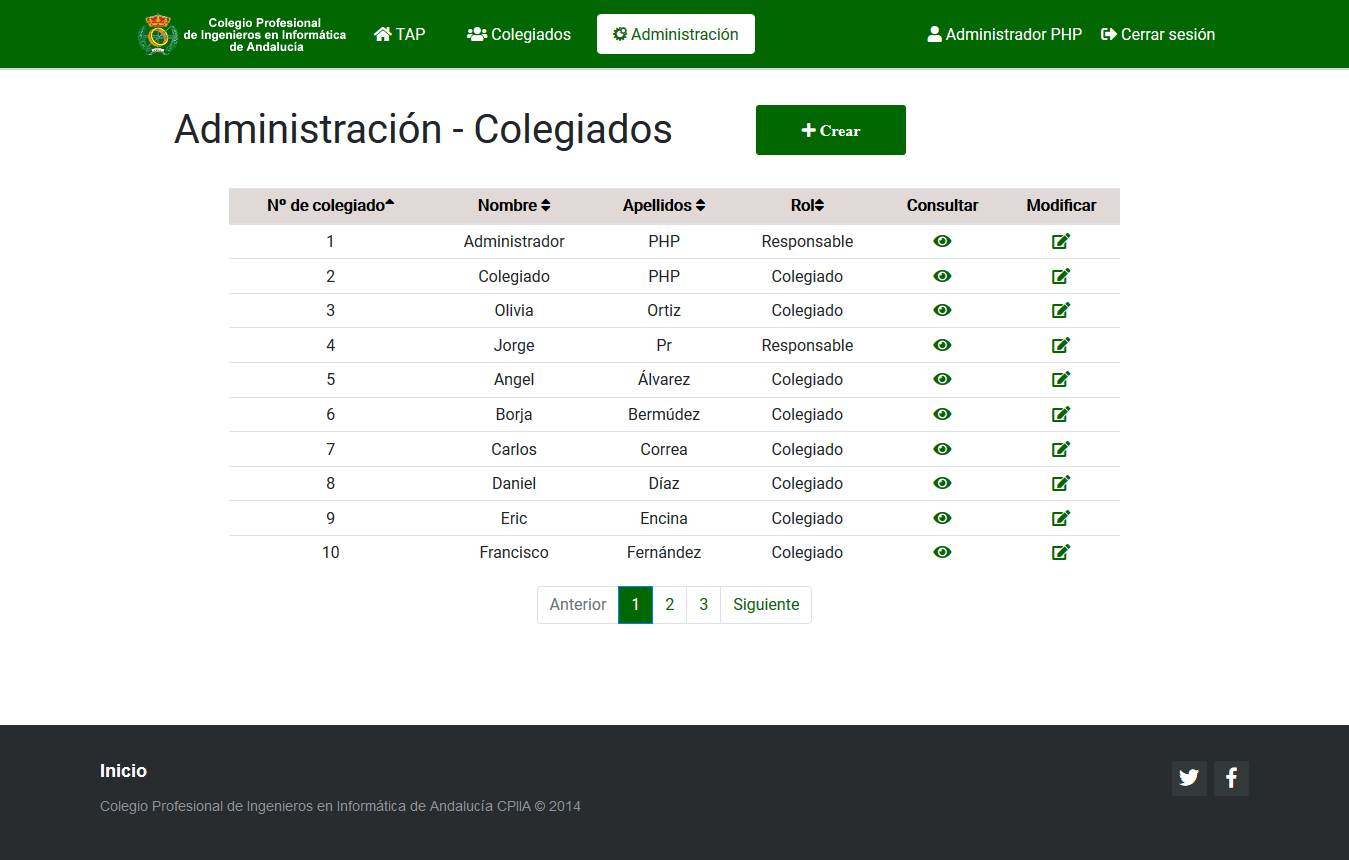
\includegraphics[width=150mm]{Web/Admin_Colegiados.png}
  \caption{Administración de Colegiados}
  \label{fig:Web_Admin_Colegiados}
\end{figure}
\FloatBarrier

\begin{figure}[!htbp]
  \centering
  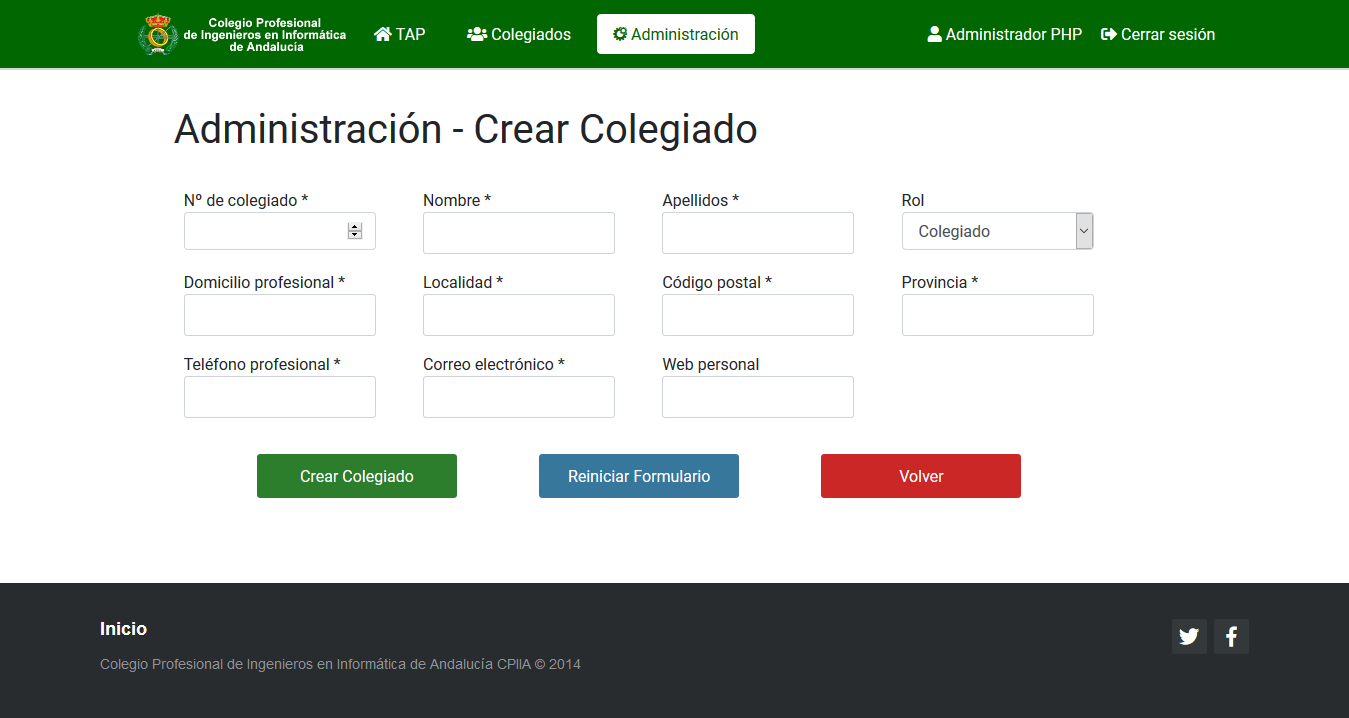
\includegraphics[width=150mm]{Web/Admin_ColegiadoCrear.png}
  \caption{Crear Colegiado}
  \label{fig:Web_Admin_ColegiadoCrear}
\end{figure}
\FloatBarrier

\begin{figure}[!htbp]
  \centering
  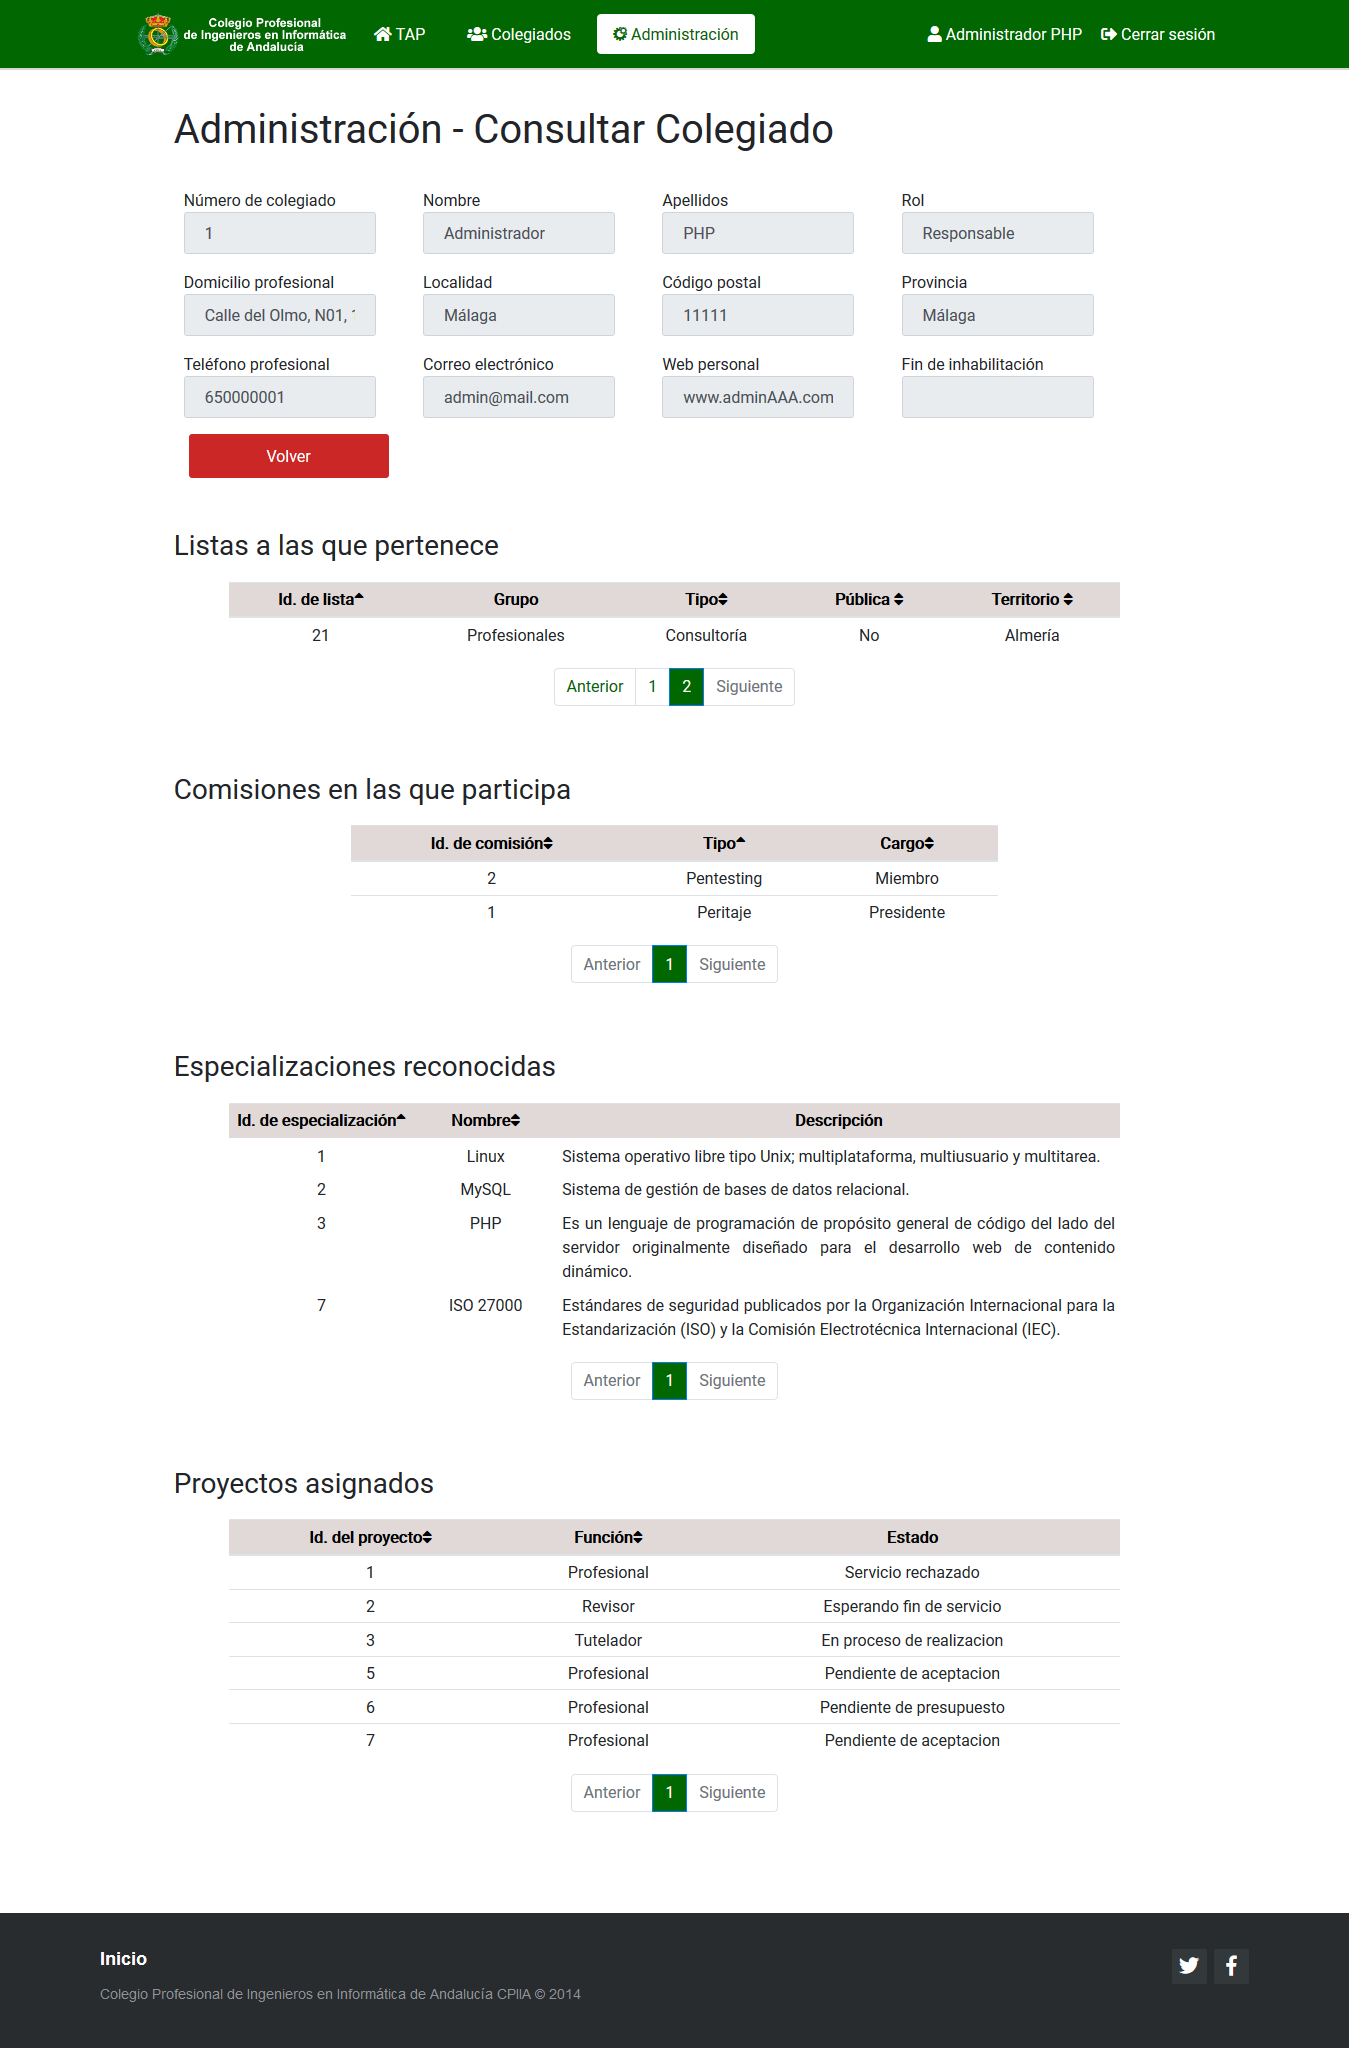
\includegraphics[width=140mm]{Web/Admin_ColegiadoConsultar.png}
  \caption{Consultar Colegiado}
  \label{fig:Web_Admin_ColegiadoConsultar}
\end{figure}
\FloatBarrier

\begin{figure}[!htbp]
  \centering
  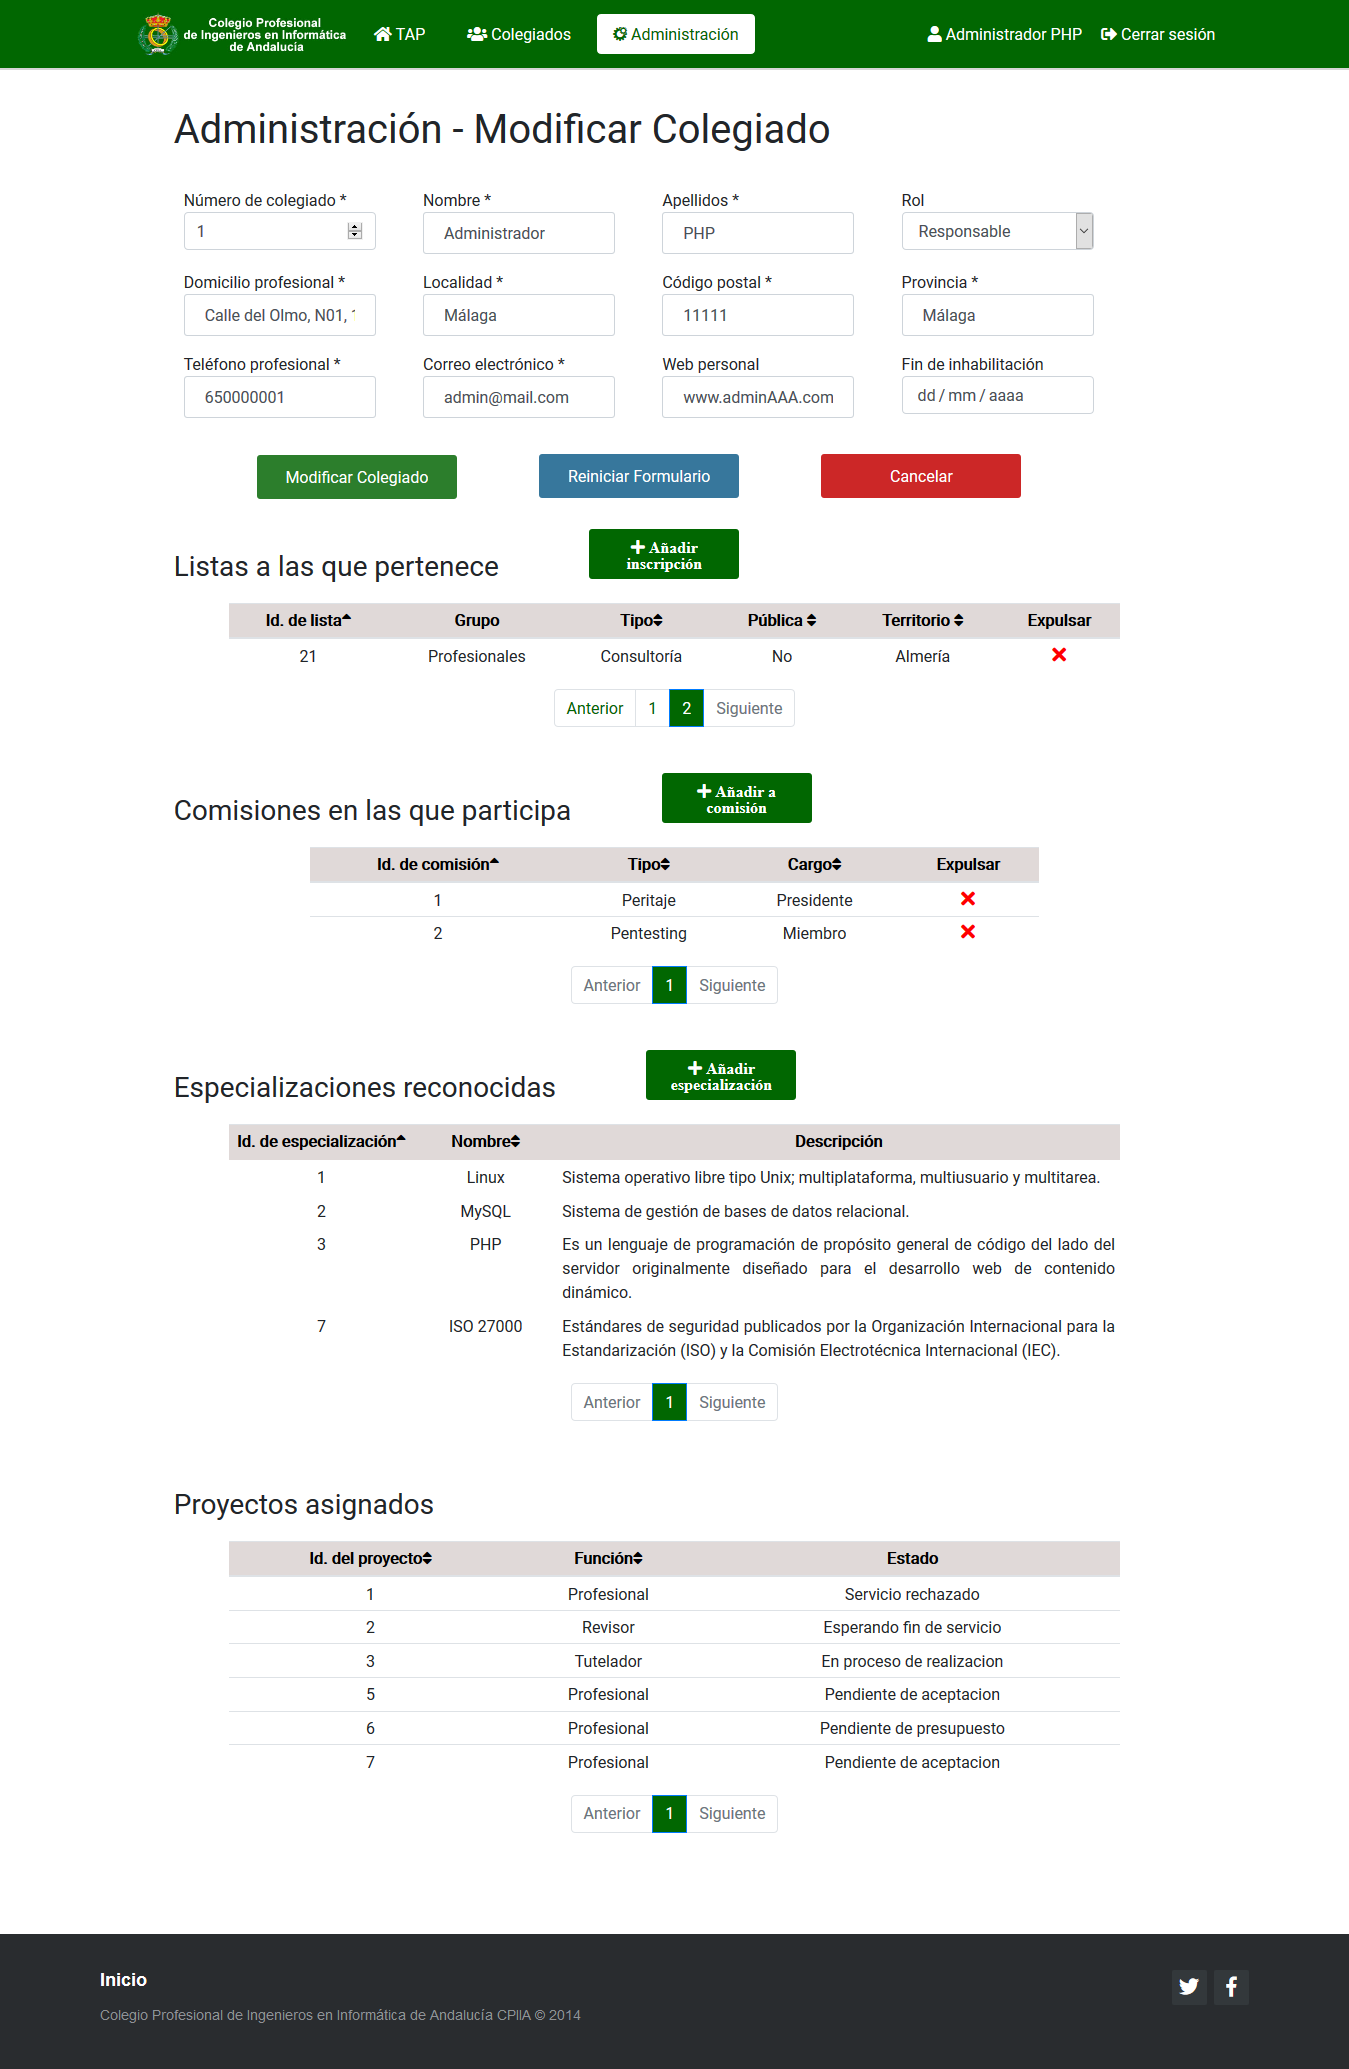
\includegraphics[width=140mm]{Web/Admin_ColegiadoModificar.png}
  \caption{Modificar Colegiado}
  \label{fig:Web_Admin_ColegiadoModificar}
\end{figure}
\FloatBarrier

Desde la vista de ``Modificar Colegiado'' (\textbf{\hyperref[fig:Web_Admin_ColegiadoModificar]{Figura 6.\arabic{figura_manual}}}) será posible establecer la fecha de inhabilitación del colegiado, lo que lo expulsará de todas las listas y comisiones a las que pertenezca. Además, se podrá acceder a:
\begin{itemize}
  \item \addtocounter{figura_manual}{1} Añadir inscripciones en listas al colegiado, en la vista ``Inscribir Colegiado en Lista'' (\textbf{\hyperref[fig:Web_Admin_ColegiadoInscribirLista]{Figura 6.\arabic{figura_manual}}}).
  \item \addtocounter{figura_manual}{1} Incluir a colegiados en comisiones de TAP, en ``Incluir Colegiado en una Comisión de TAP'' (\textbf{\hyperref[fig:Web_Admin_ColegiadoIncluirComision]{Figura 6.\arabic{figura_manual}}}).
  \item \addtocounter{figura_manual}{1} Registrar las especializaciones acreditadas por el colegiado, en la vista ``Asignar Especialización a Colegiado'' (\textbf{\hyperref[fig:Web_Admin_ColegiadoAsignarEspecializacion]{Figura 6.\arabic{figura_manual}}}).
\end{itemize}

\begin{figure}[!htbp]
  \centering
  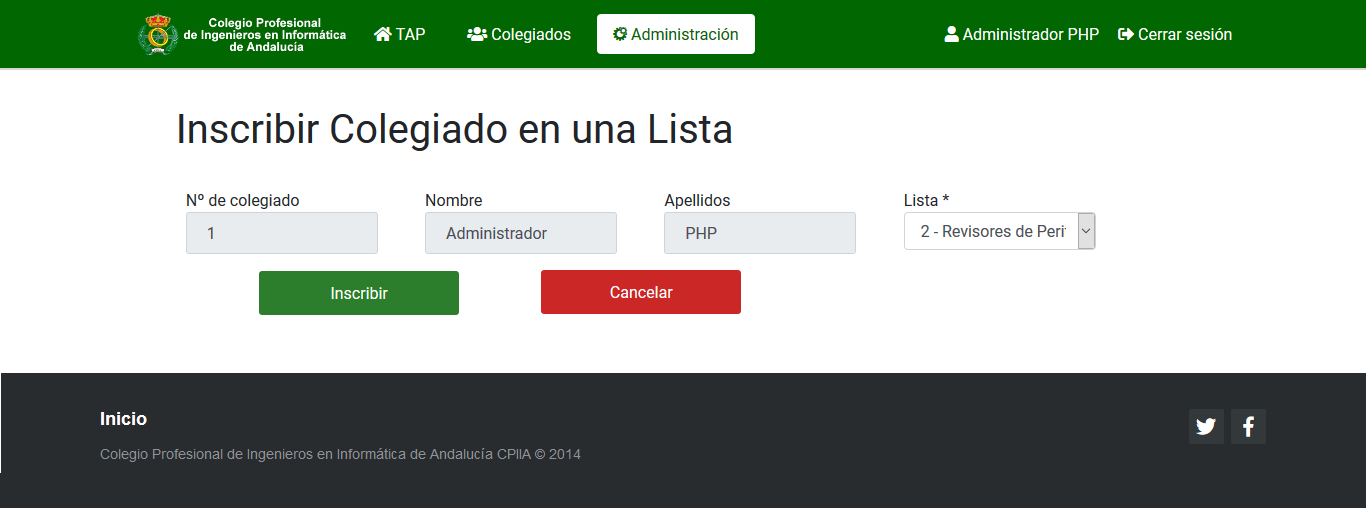
\includegraphics[width=150mm]{Web/Admin_ColegiadoInscribirLista.png}
  \caption{Inscribir Colegiado en Lista}
  \label{fig:Web_Admin_ColegiadoInscribirLista}
\end{figure}
\FloatBarrier

\begin{figure}[!htbp]
  \centering
  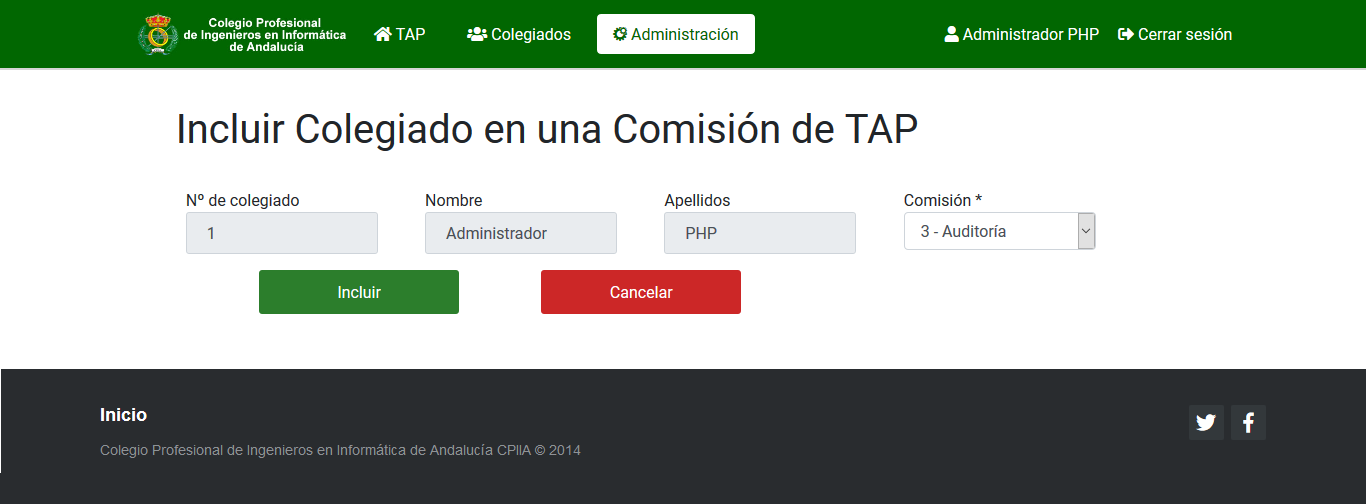
\includegraphics[width=150mm]{Web/Admin_ColegiadoIncluirComision.png}
  \caption{Incluir Colegiado en una Comisión de TAP}
  \label{fig:Web_Admin_ColegiadoIncluirComision}
\end{figure}
\FloatBarrier

\begin{figure}[!htbp]
  \centering
  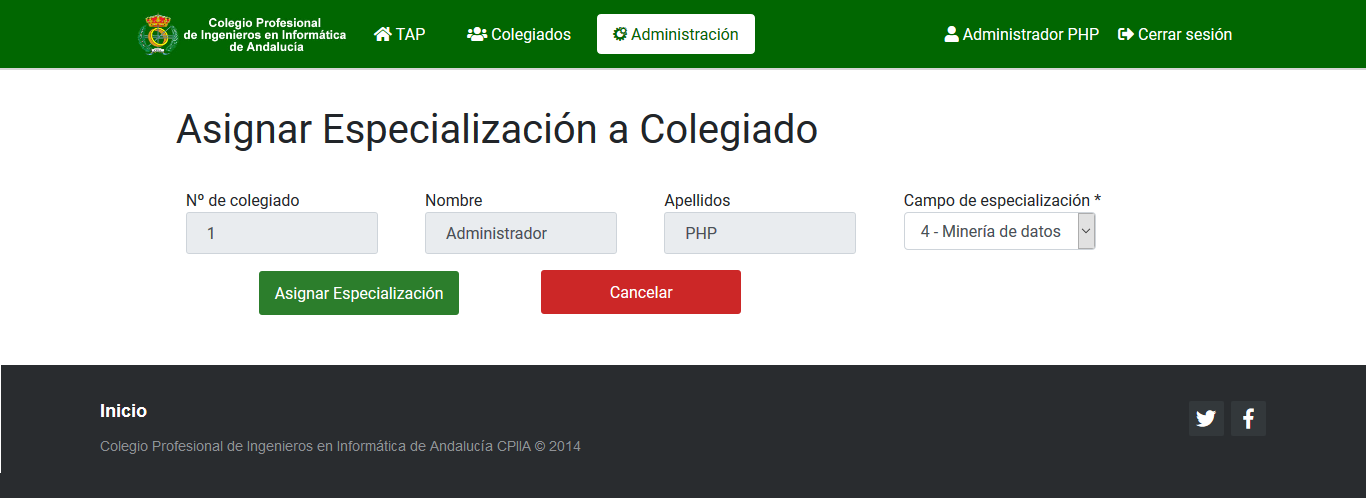
\includegraphics[width=150mm]{Web/Admin_ColegiadoAsignarEspecializacion.png}
  \caption{Asignar Especialización a Colegiado}
  \label{fig:Web_Admin_ColegiadoAsignarEspecializacion}
\end{figure}
\FloatBarrier

\addtocounter{figura_manual}{1} En cuanto a la administración de listas, accesible en la vista ``Administración de Listas'' (\textbf{\hyperref[fig:Web_Admin_Listas]{Figura 6.\arabic{figura_manual}}}), será posible filtrar las listas por tipo de lista, si es de profesionales o revisores, si es pública o no y por territorio.\addtocounter{figura_manual}{1}  También permitirá acceder a la creación (\textbf{\hyperref[fig:Web_Admin_ListaCrear]{Figura 6.\arabic{figura_manual}}}),\addtocounter{figura_manual}{1}  consulta (\textbf{\hyperref[fig:Web_Admin_ListaConsultar]{Figura 6.\arabic{figura_manual}}})\addtocounter{figura_manual}{1}  y modificación (\textbf{\hyperref[fig:Web_Admin_ListaModificar]{Figura 6.\arabic{figura_manual}}}) de listas. Para actualizar el estado de las inscripciones de los colegiados en una lista será necesario acceder a la vista de modificación de dicha lista.
\begin{figure}[!htbp]
  \centering
  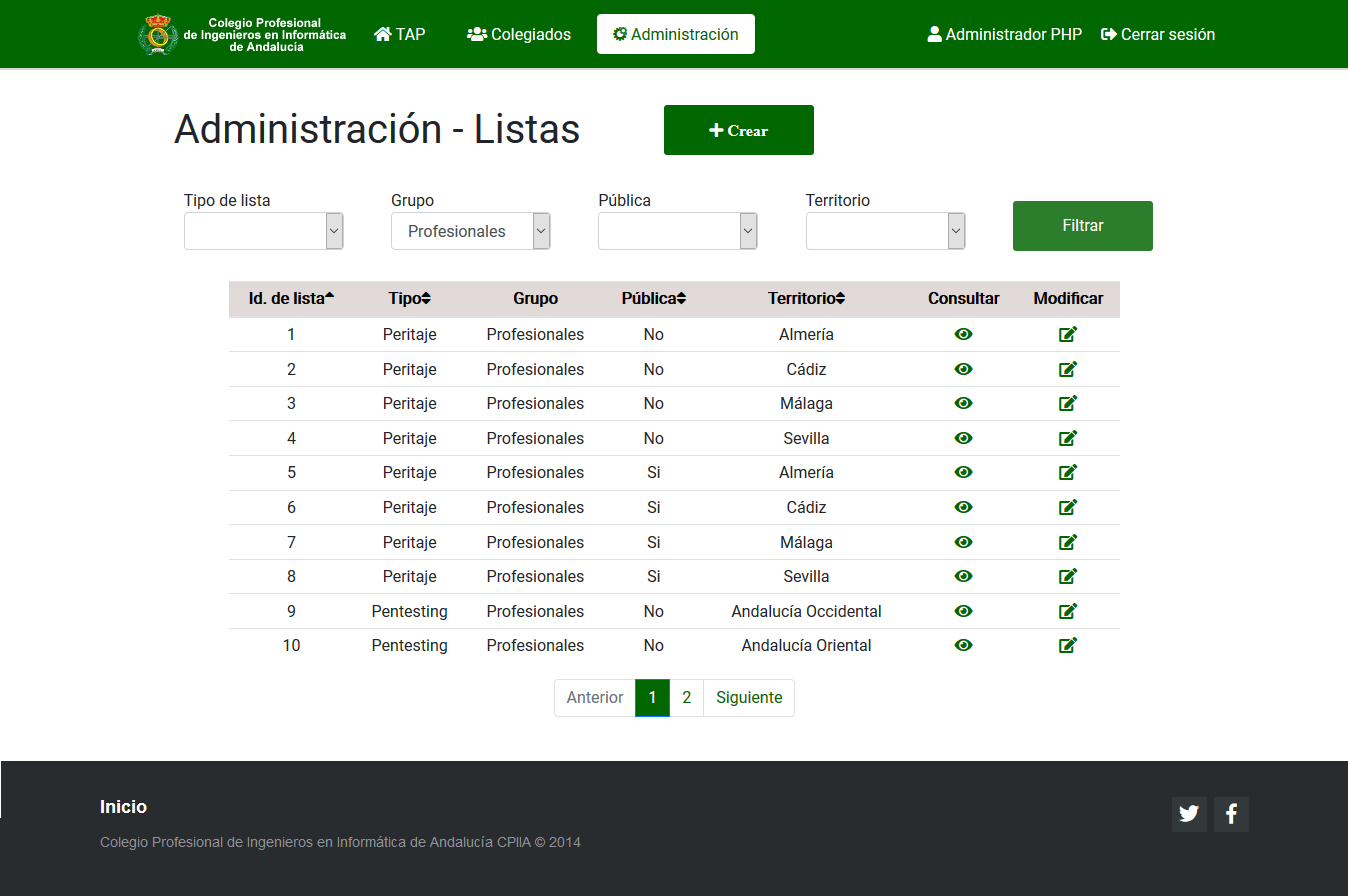
\includegraphics[width=150mm]{Web/Admin_Listas.png}
  \caption{Administración de Listas}
  \label{fig:Web_Admin_Listas}
\end{figure}
\FloatBarrier

\begin{figure}[!h]
  \centering
  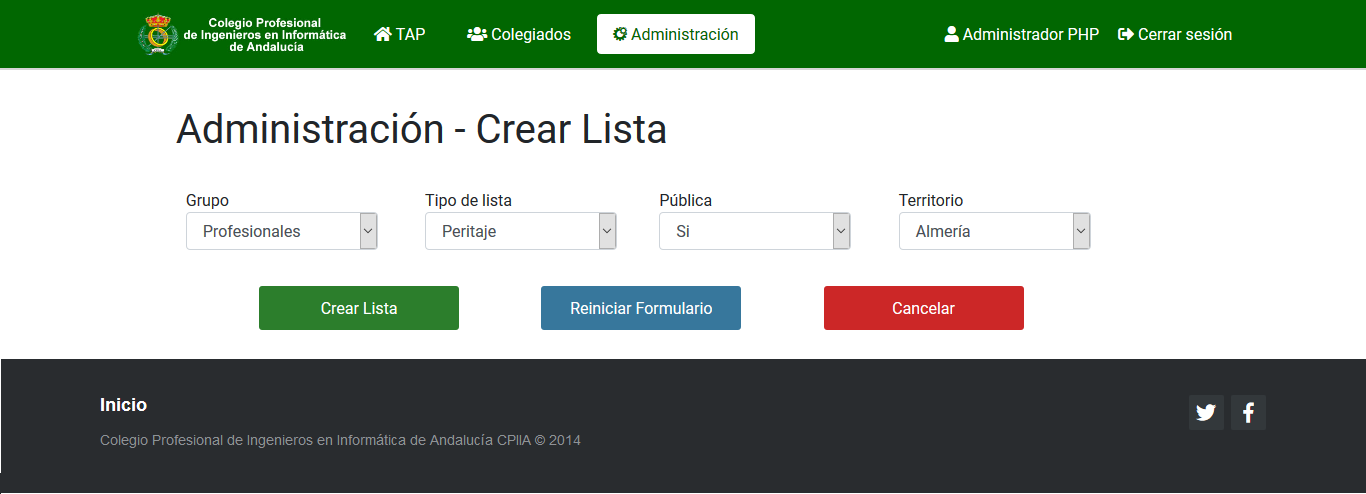
\includegraphics[width=150mm]{Web/Admin_ListaCrear.png}
  \caption{Crear Lista}
  \label{fig:Web_Admin_ListaCrear}
\end{figure}
\FloatBarrier

\begin{figure}[!h]
  \centering
  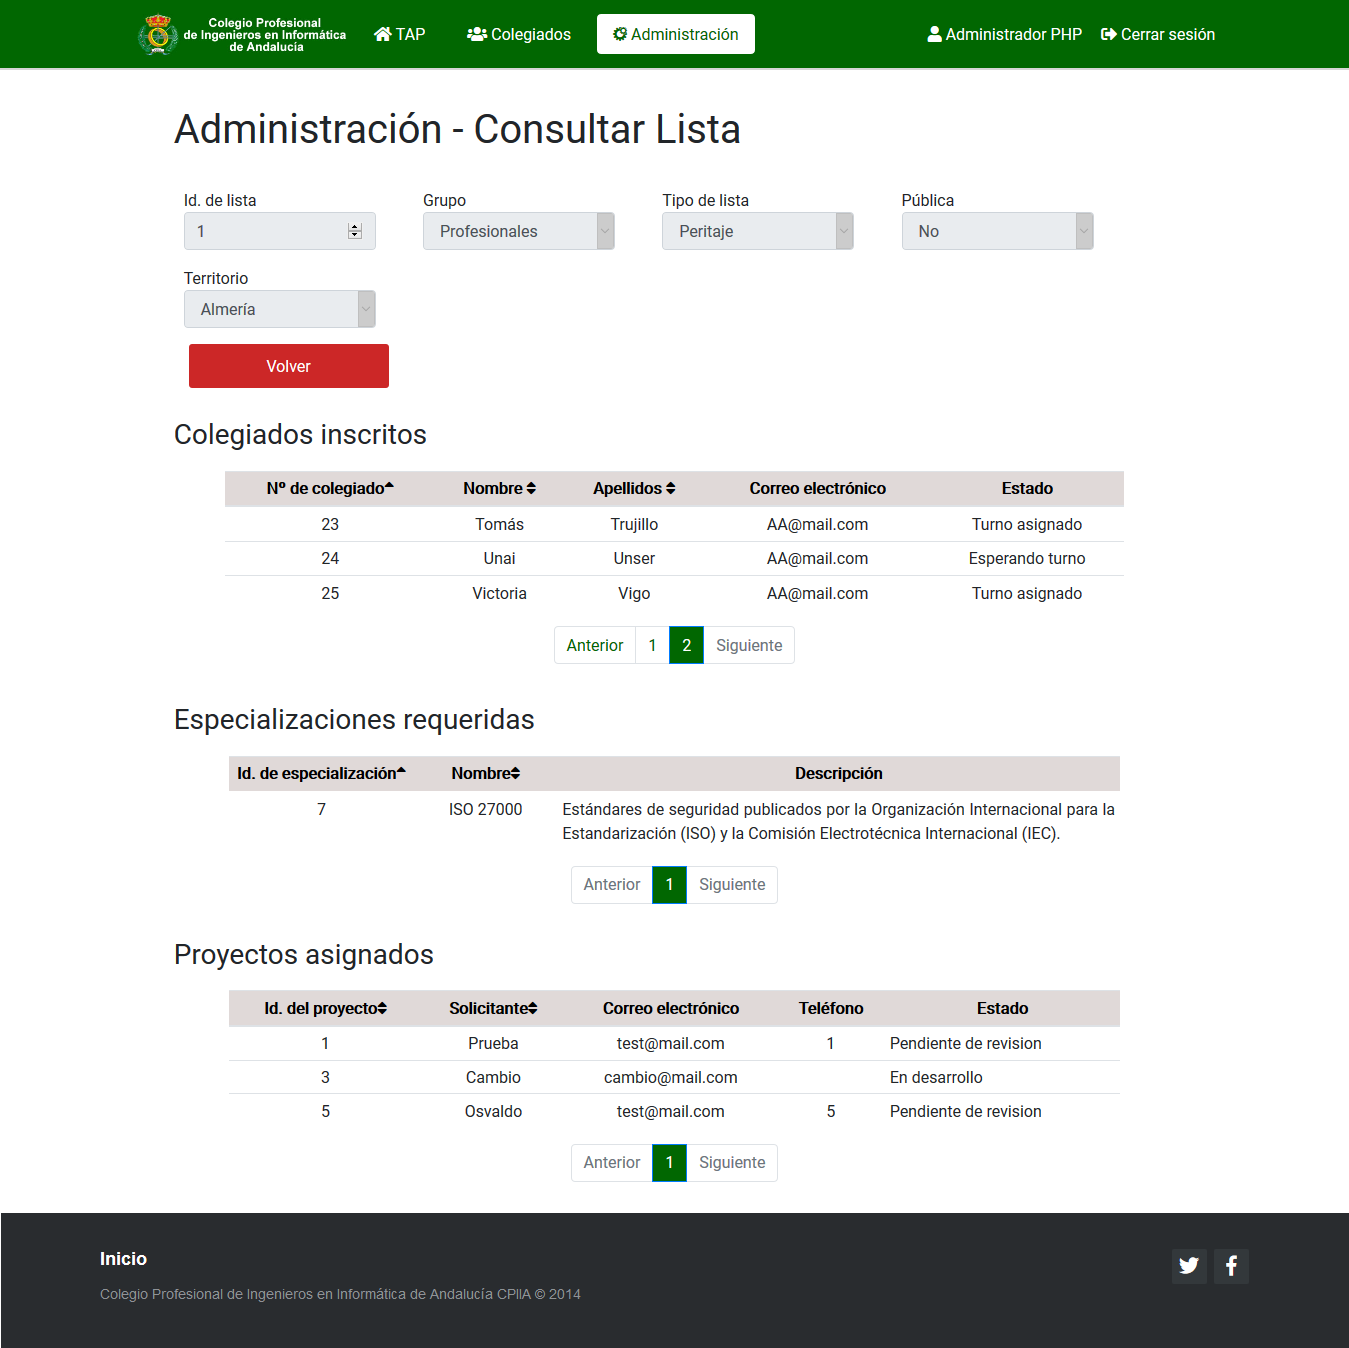
\includegraphics[width=150mm]{Web/Admin_ListaConsultar.png}
  \caption{Consultar Lista}
  \label{fig:Web_Admin_ListaConsultar}
\end{figure}
\FloatBarrier

\begin{figure}[!p]
  \centering
  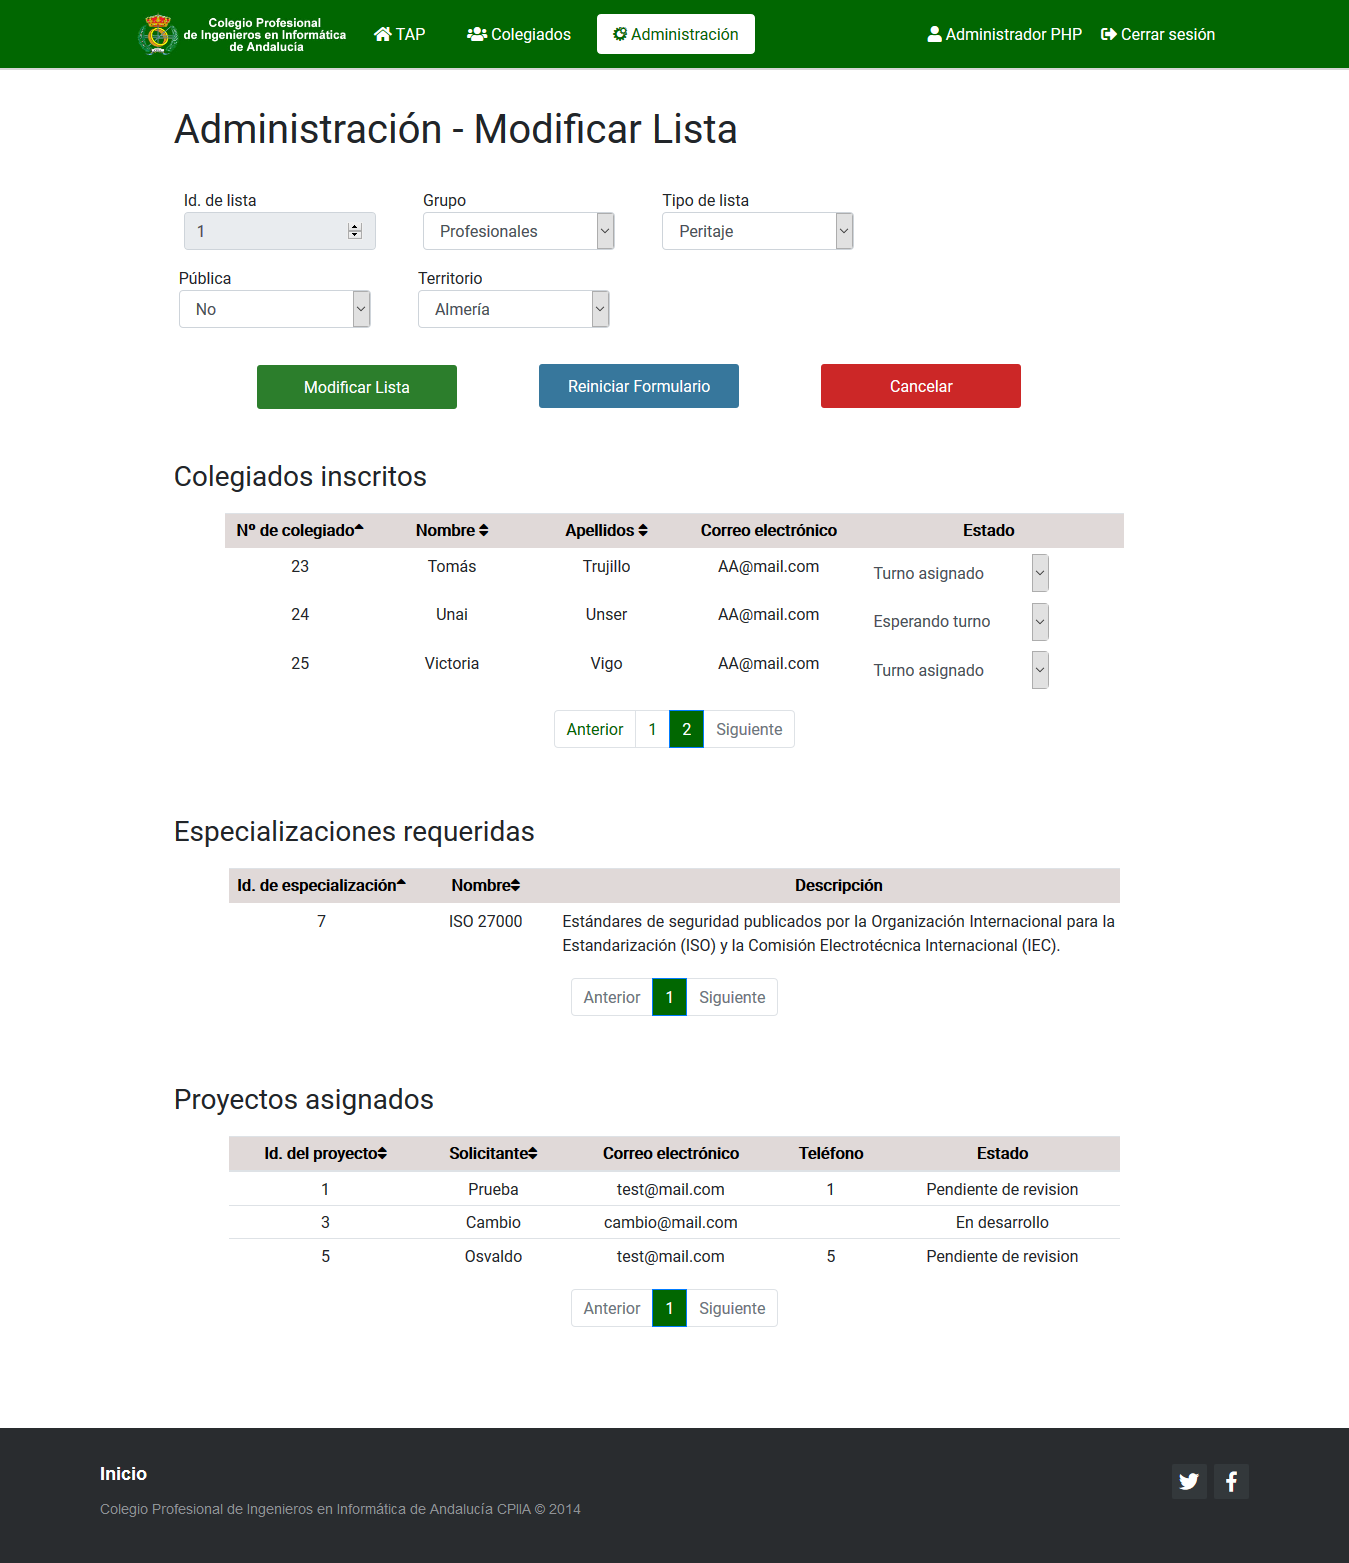
\includegraphics[width=150mm]{Web/Admin_ListaModificar.png}
  \caption{Modificar Lista}
  \label{fig:Web_Admin_ListaModificar}
\end{figure}
\FloatBarrier

\newpage~
\addtocounter{figura_manual}{1} Relativo a la administración de tipos de lista (\textbf{\hyperref[fig:Web_Admin_TiposLista]{Figura 6.\arabic{figura_manual}}}),\addtocounter{figura_manual}{1} se podrá crear nuevos tipos (\textbf{\hyperref[fig:Web_Admin_TipoListaCrear]{Figura 6.\arabic{figura_manual}}})\addtocounter{figura_manual}{1} y consultar (\textbf{\hyperref[fig:Web_Admin_TipoListaConsultar]{Figura 6.\arabic{figura_manual}}})\addtocounter{figura_manual}{1} y modificar (\textbf{\hyperref[fig:Web_Admin_TipoListaModificar]{Figura 6.\arabic{figura_manual}}}) los ya existentes. Algunas observaciones a tener en cuenta para la gestión de tipos de lista son:
\begin{itemize}
  \item \addtocounter{figura_manual}{1} Para crear un nuevo tipo de lista, es necesario que exista anteriormente una comisión de TAP que no haya sido asignada a otro tipo.
  \item Desde las vistas ``Crear Tipo de Lista'' y ``Modificar Tipo de Lista'' se podrá establecer el periodo vacacional de todas las listas pertenecientes a ese tipo.
  \item Desde ``Modificar Tipo de Lista'' se podrá acceder a la vista para requerir conocimientos en una especialización para poder inscribirse en la lista (\textbf{\hyperref[fig:Web_Admin_TipoListaRequerirEspecializacion]{Figura 6.\arabic{figura_manual}}}).
\end{itemize}

\begin{figure}[!htbp]
  \centering
  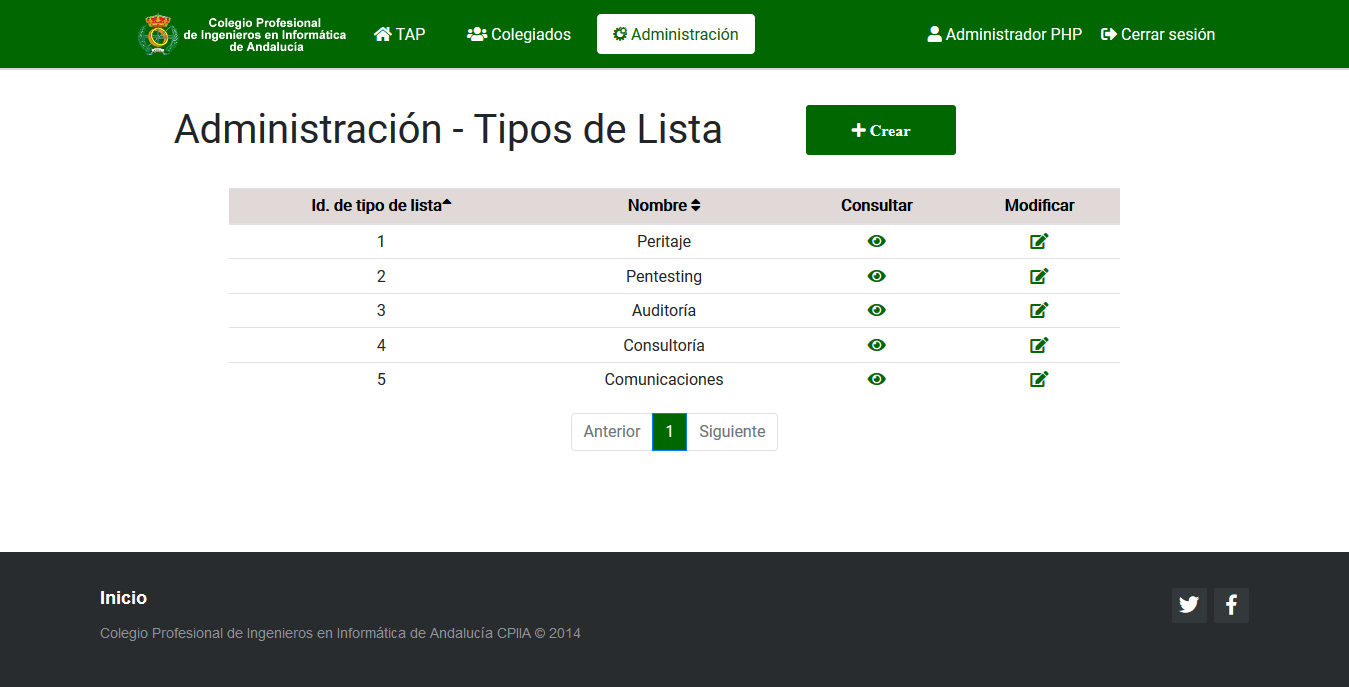
\includegraphics[width=150mm]{Web/Admin_TiposLista.png}
  \caption{Administración de Tipos de Lista}
  \label{fig:Web_Admin_TiposLista}
\end{figure}
\FloatBarrier

\begin{figure}[!htbp]
  \centering
  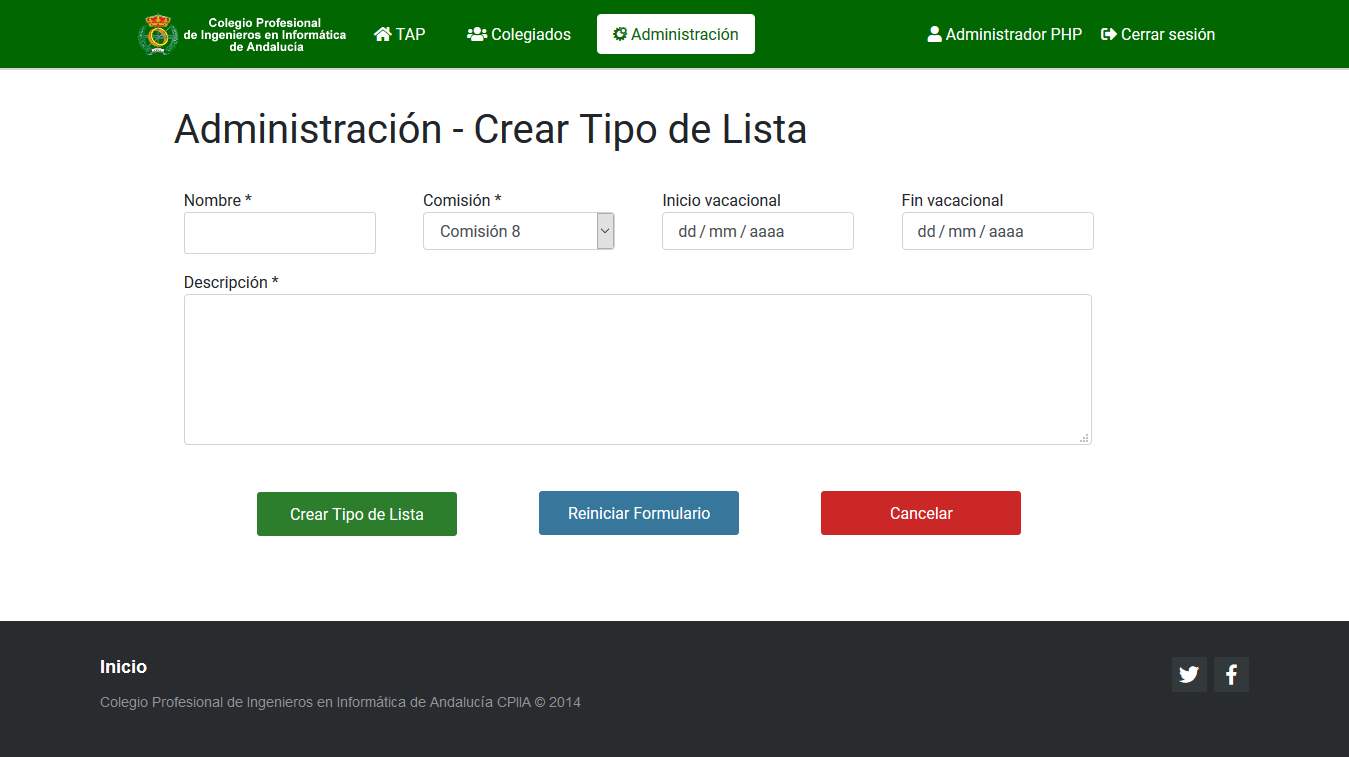
\includegraphics[width=150mm]{Web/Admin_TipoListaCrear.png}
  \caption{Crear Tipo de Lista}
  \label{fig:Web_Admin_TipoListaCrear}
\end{figure}
\FloatBarrier

\begin{figure}[!htbp]
  \centering
  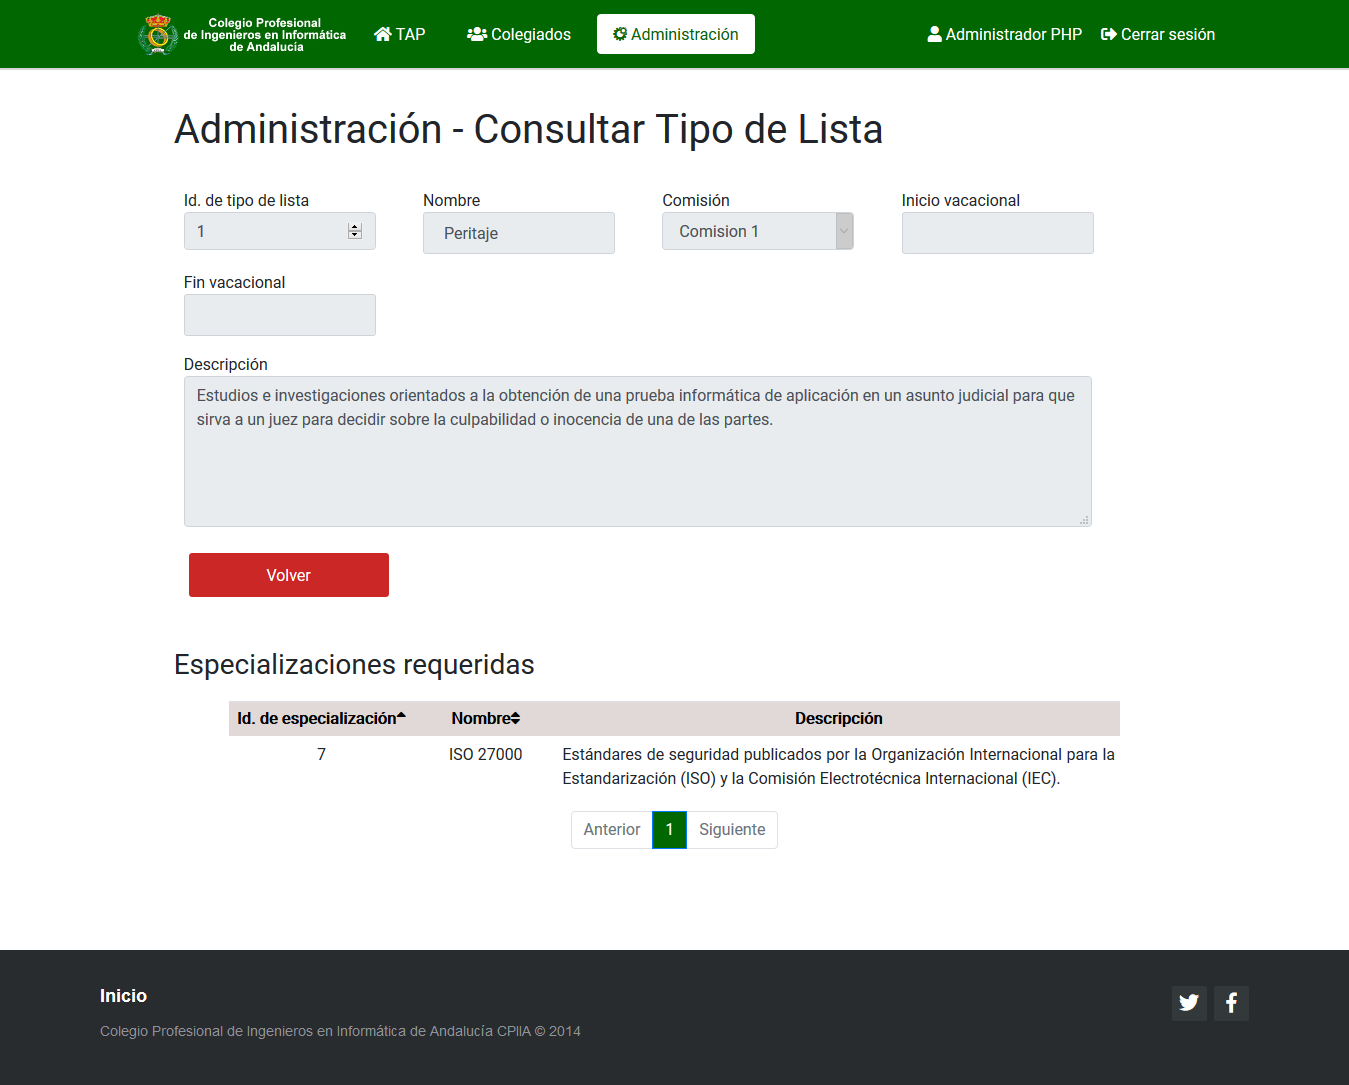
\includegraphics[width=150mm]{Web/Admin_TipoListaConsultar.png}
  \caption{Consultar Tipo de Lista}
  \label{fig:Web_Admin_TipoListaConsultar}
\end{figure}
\FloatBarrier

\begin{figure}[!htbp]
  \centering
  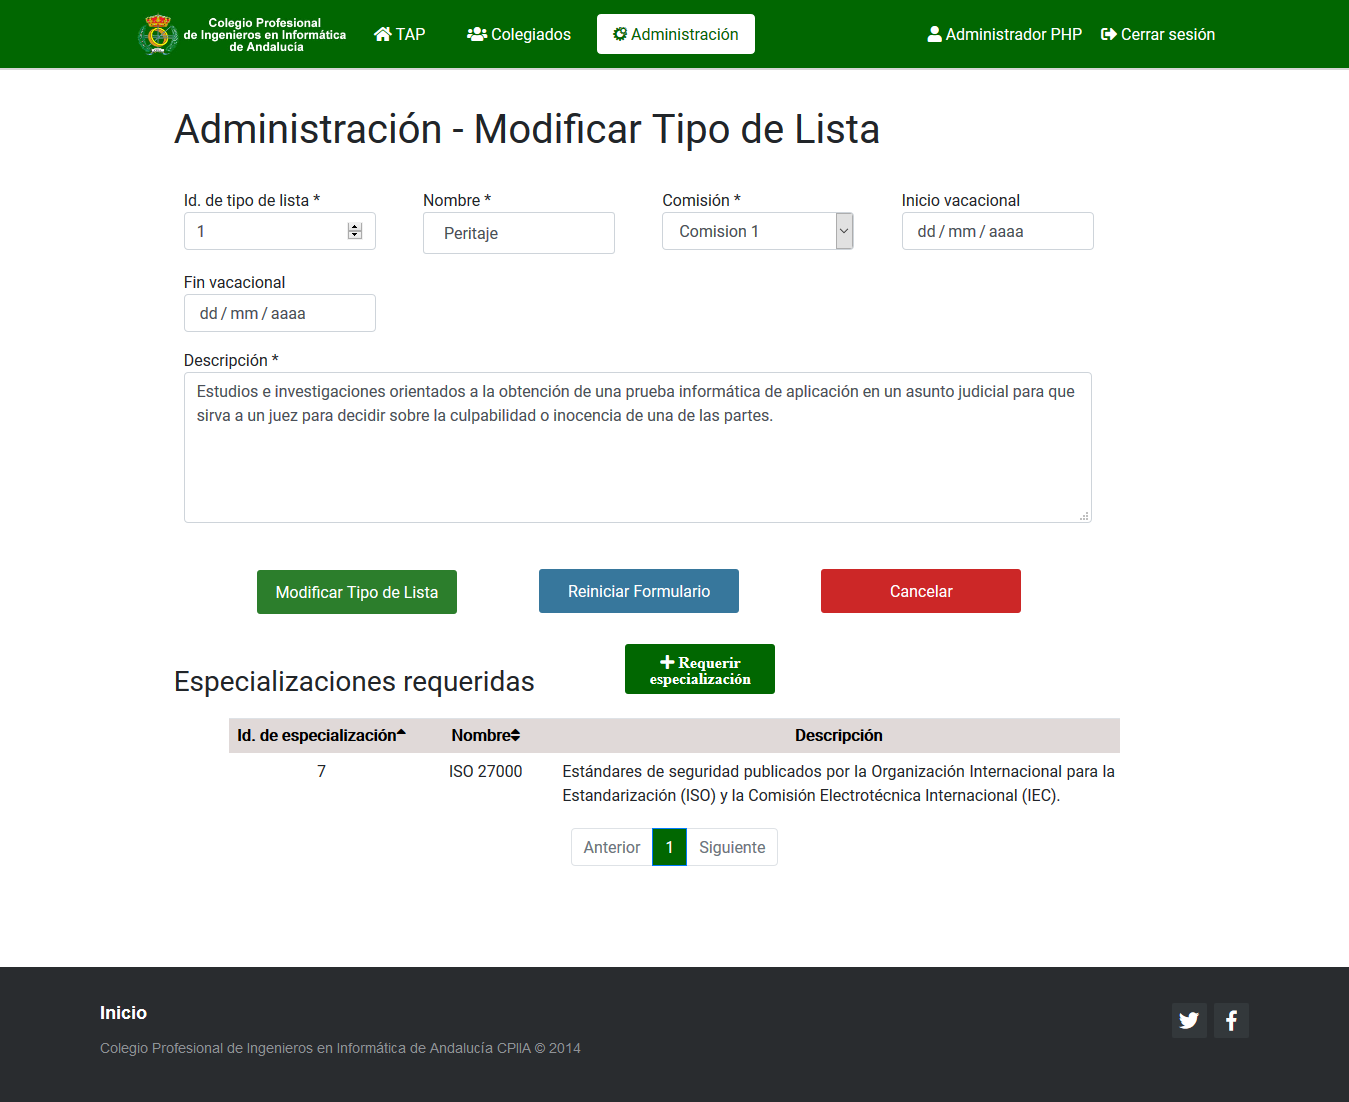
\includegraphics[width=150mm]{Web/Admin_TipoListaModificar.png}
  \caption{Modificar Tipo de Lista}
  \label{fig:Web_Admin_TipoListaModificar}
\end{figure}
\FloatBarrier

\begin{figure}[!htbp]
  \centering
  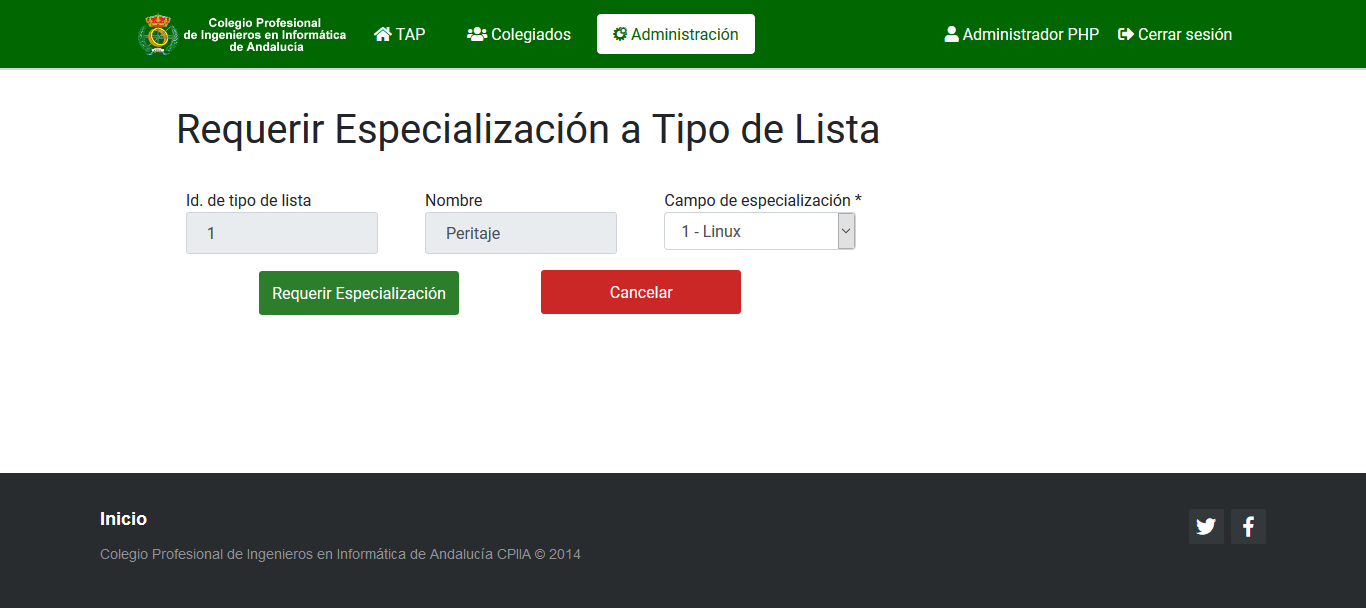
\includegraphics[width=150mm]{Web/Admin_TipoListaRequerirEspecializacion.png}
  \caption{Requerir Especialización a Tipo de Lista}
  \label{fig:Web_Admin_TipoListaRequerirEspecializacion}
\end{figure}
\FloatBarrier

\pagebreak \addtocounter{figura_manual}{1} La ``Administración de Especializaciones''  (\textbf{\hyperref[fig:Web_Admin_Especializaciones]{Figura 6.\arabic{figura_manual}}}),\addtocounter{figura_manual}{1} permite crear (\textbf{\hyperref[fig:Web_Admin_EspecializacionCrear]{Figura 6.\arabic{figura_manual}}}), \addtocounter{figura_manual}{1}, consultar (\textbf{\hyperref[fig:Web_Admin_EspecializacionConsultar]{Figura 6.\arabic{figura_manual}}})\addtocounter{figura_manual}{1} y modificar (\textbf{\hyperref[fig:Web_Admin_EspecializacionModificar]{Figura 6.\arabic{figura_manual}}}) especializaciones.
\begin{figure}[!htbp]
  \centering
  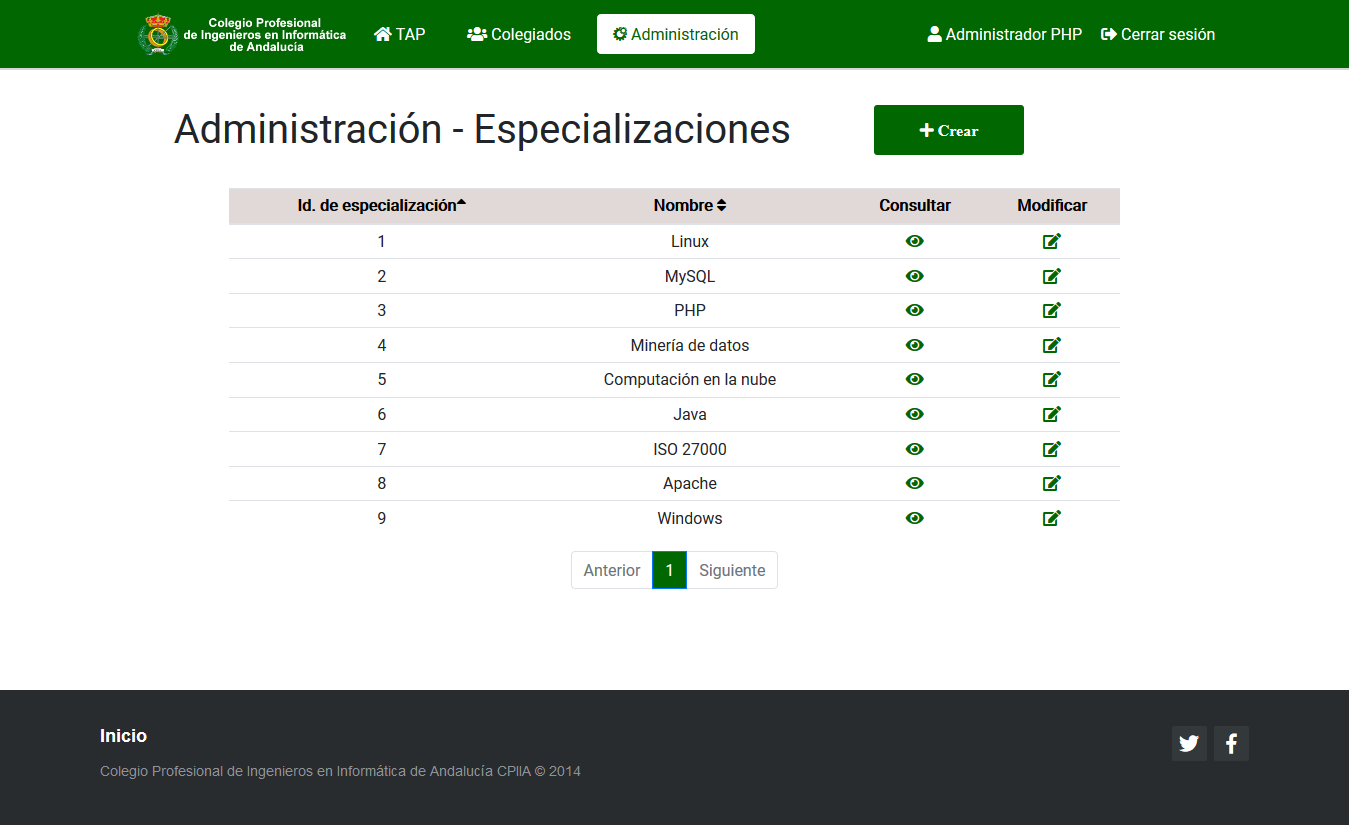
\includegraphics[width=150mm]{Web/Admin_Especializaciones.png}
  \caption{Administración de Especializaciones}
  \label{fig:Web_Admin_Especializaciones}
\end{figure}
\FloatBarrier

\begin{figure}[!htbp]
  \centering
  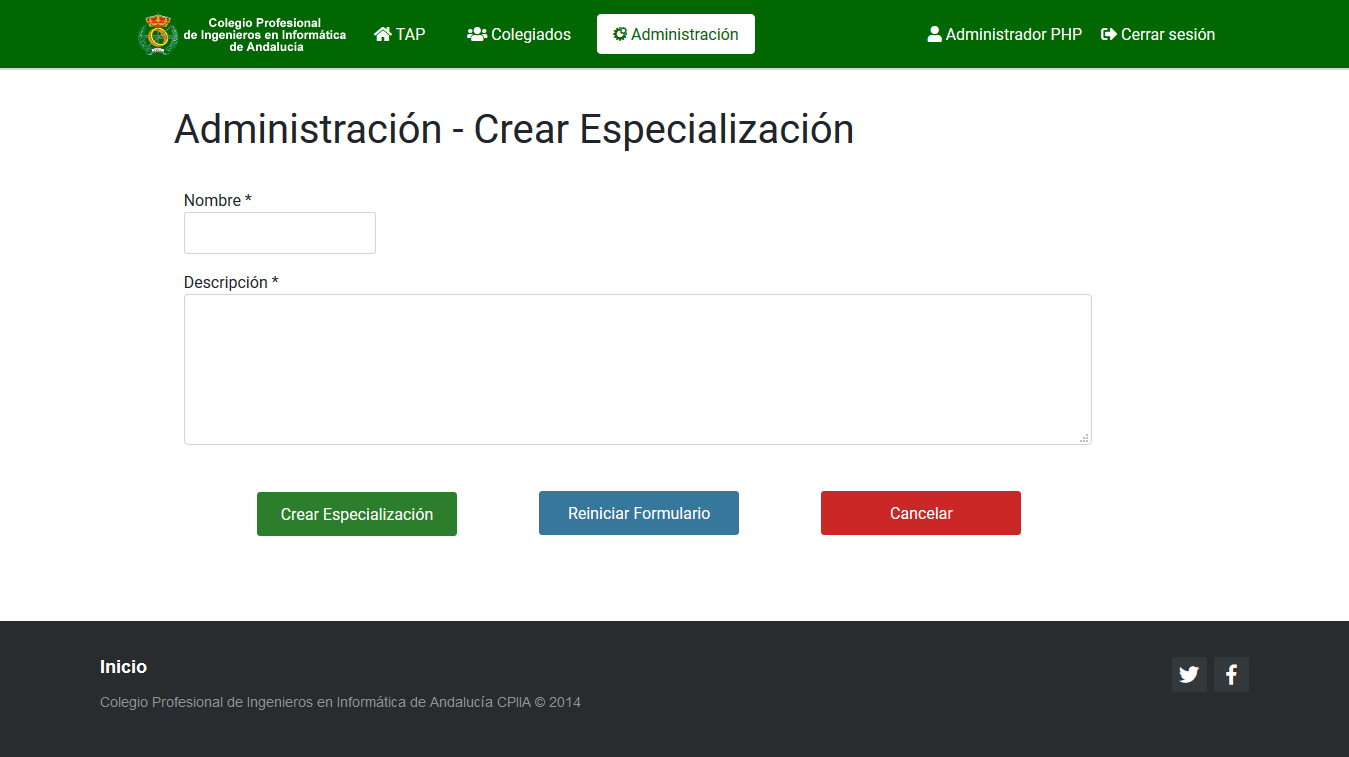
\includegraphics[width=150mm]{Web/Admin_EspecializacionCrear.png}
  \caption{Crear Especialización}
  \label{fig:Web_Admin_EspecializacionCrear}
\end{figure}
\FloatBarrier

\begin{figure}[!htbp]
  \centering
  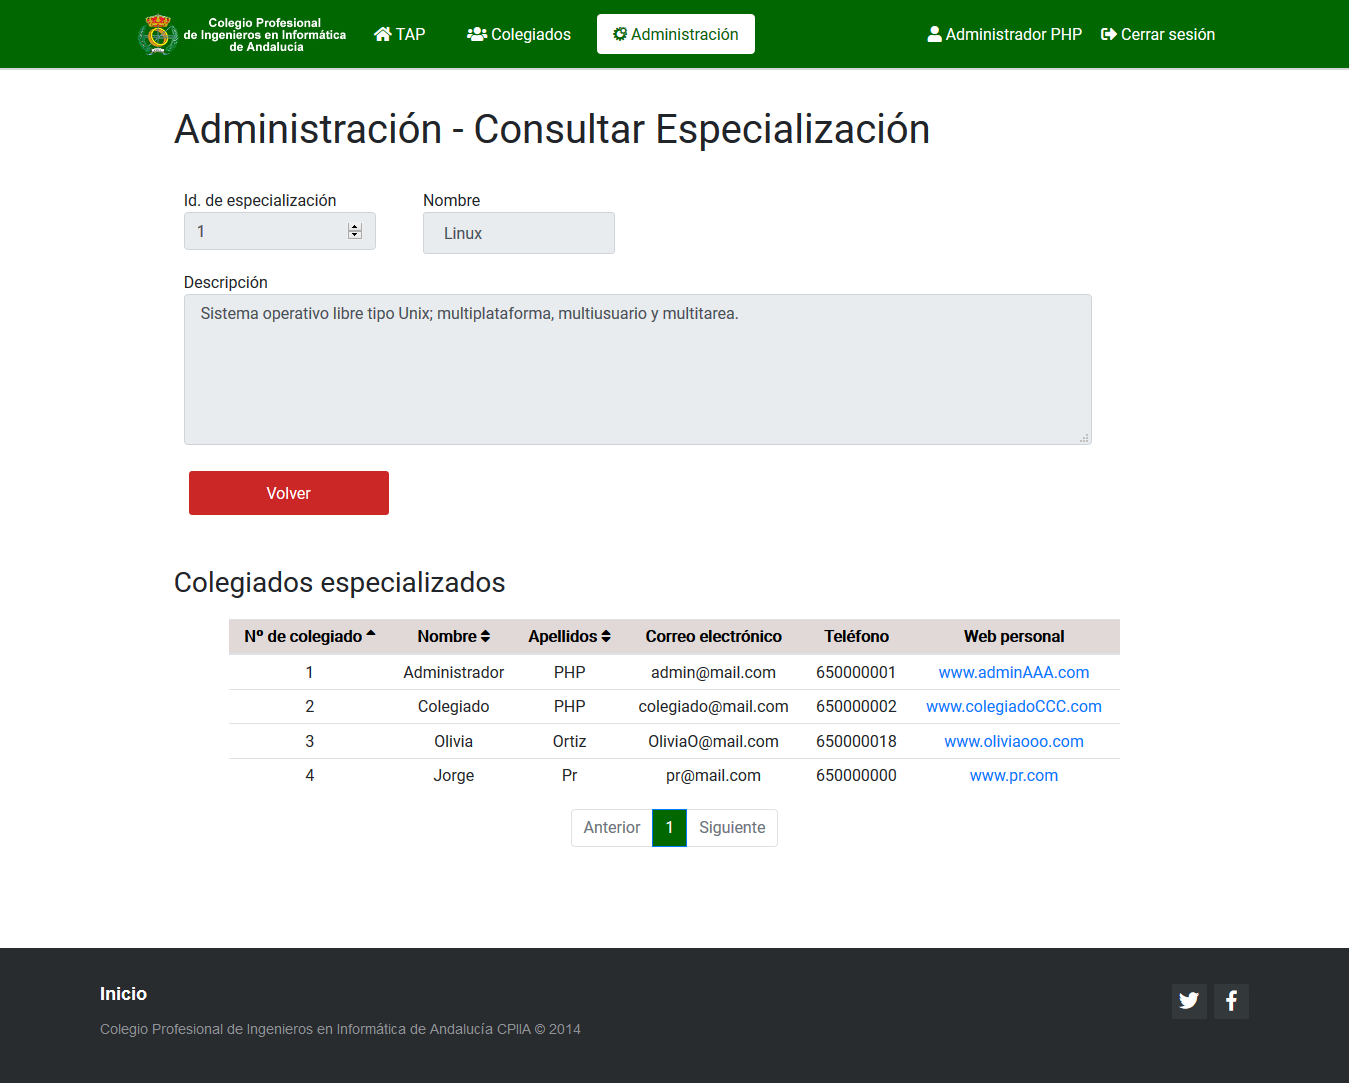
\includegraphics[width=150mm]{Web/Admin_EspecializacionConsultar.png}
  \caption{Consultar Especialización}
  \label{fig:Web_Admin_EspecializacionConsultar}
\end{figure}
\FloatBarrier

\begin{figure}[!htbp]
  \centering
  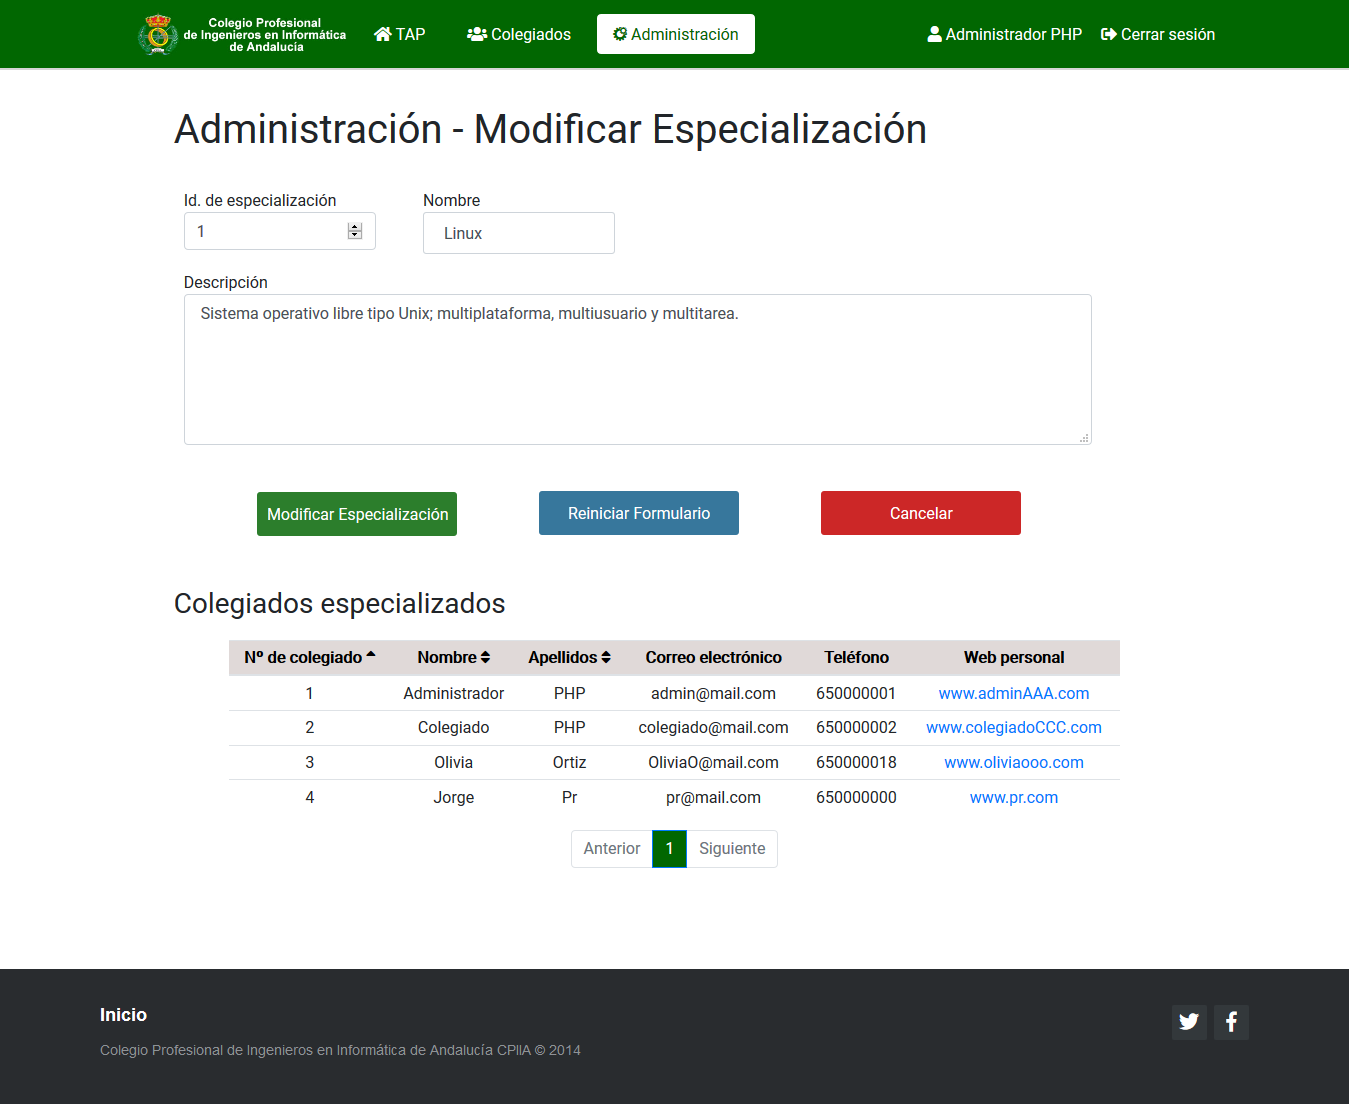
\includegraphics[width=150mm]{Web/Admin_EspecializacionModificar.png}
  \caption{Modificar Especialización}
  \label{fig:Web_Admin_EspecializacionModificar}
\end{figure}
\FloatBarrier

\addtocounter{figura_manual}{1} En cuanto a la ``Administración de Comisiones'' (\textbf{\hyperref[fig:Web_Admin_Comisiones]{Figura 6.\arabic{figura_manual}}}),\addtocounter{figura_manual}{1} permite crear, consultar (\textbf{\hyperref[fig:Web_Admin_ComisionConsultar]{Figura 6.\arabic{figura_manual}}})\addtocounter{figura_manual}{1} y modificar (\textbf{\hyperref[fig:Web_Admin_ComisionModificar]{Figura 6.\arabic{figura_manual}}}) comisiones. Algunas observaciones a tener en cuenta son:
\begin{itemize}
  \item La función de crear la comisión no lleva una vista donde introducir datos para crearla, sino que se crea directamente al pulsar el botón ``Crear'' en la vista ``Administración de Comisiones''.
  \item También en la vista ``Administración de Comisiones'', es posible eliminar aquellas comisiones que no tengan asignadas un tipo de lista.
\end{itemize}

\begin{figure}[!htbp]
  \centering
  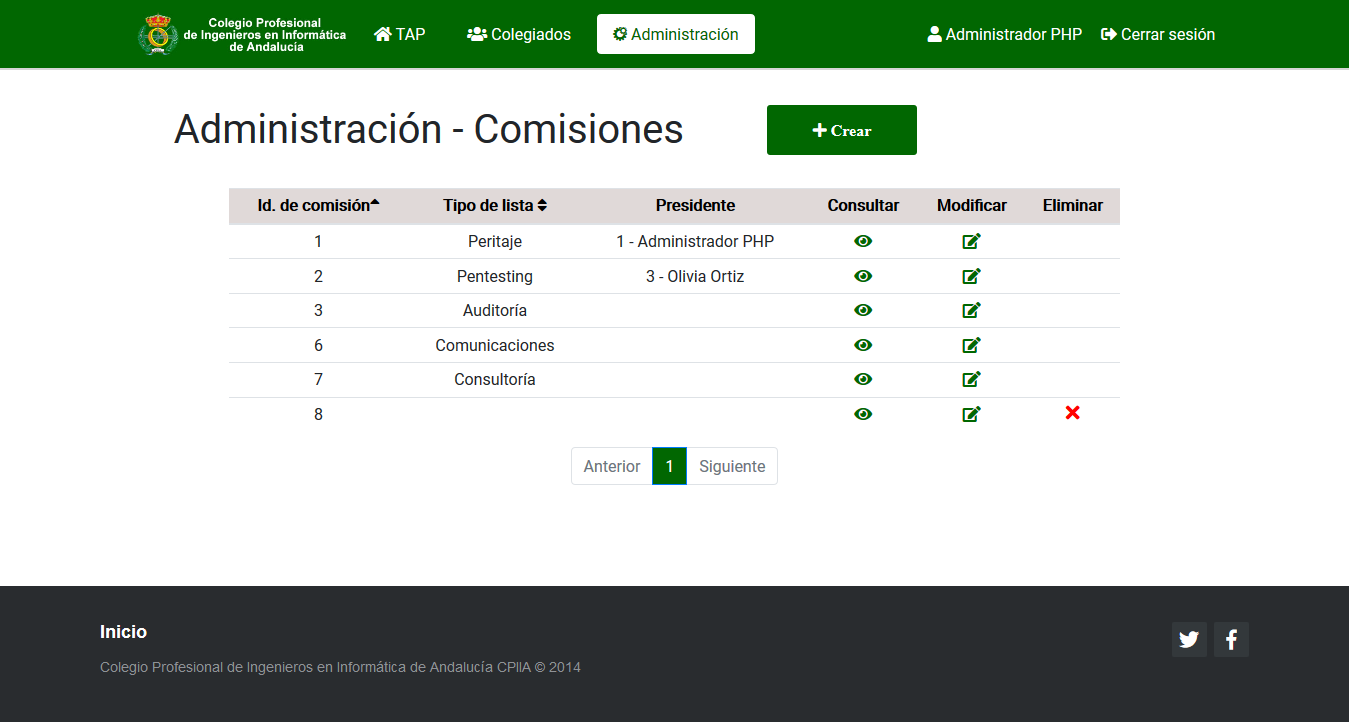
\includegraphics[width=150mm]{Web/Admin_Comisiones.png}
  \caption{Administración de Comisiones}
  \label{fig:Web_Admin_Comisiones}
\end{figure}
\FloatBarrier

\begin{figure}[!htbp]
  \centering
  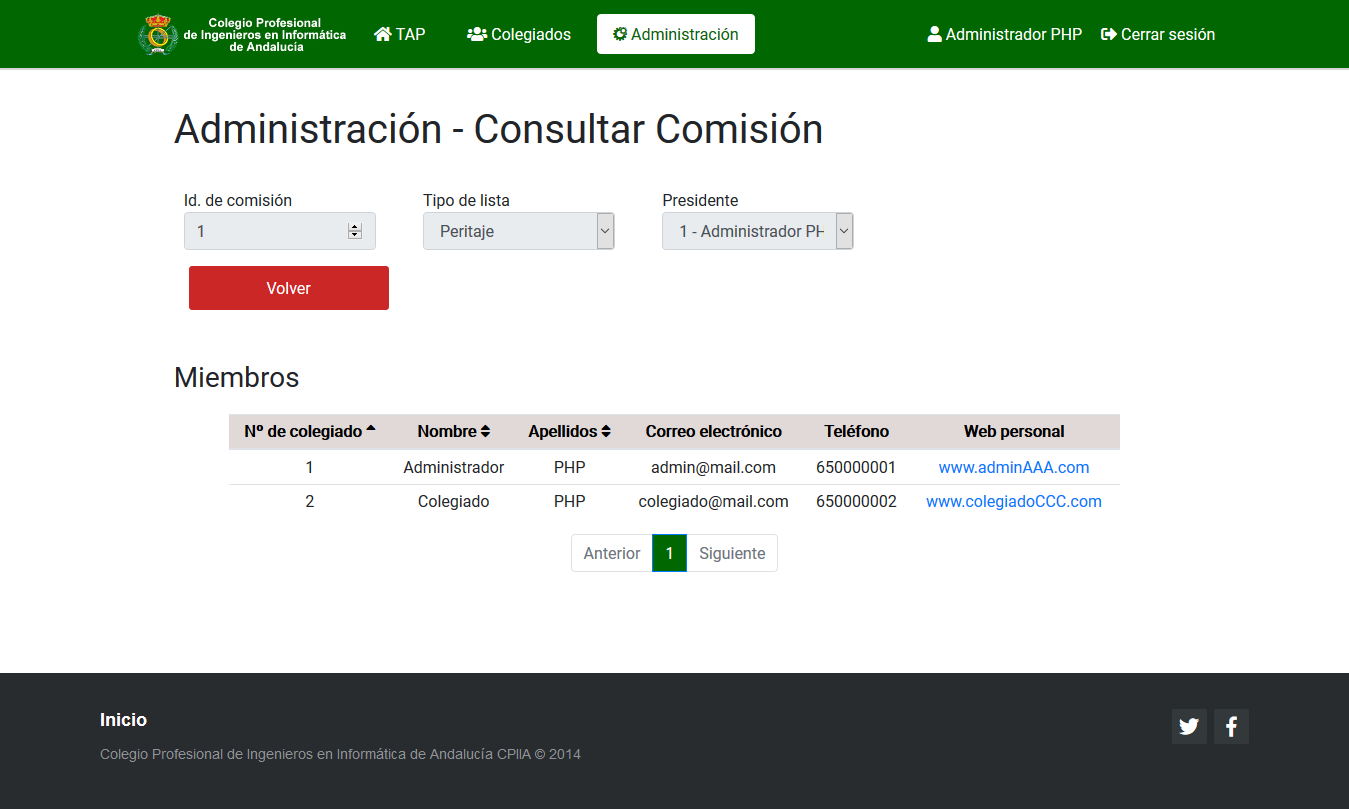
\includegraphics[width=150mm]{Web/Admin_ComisionConsultar.png}
  \caption{Consultar Comisión}
  \label{fig:Web_Admin_ComisionConsultar}
\end{figure}
\FloatBarrier

\begin{figure}[!htbp]
  \centering
  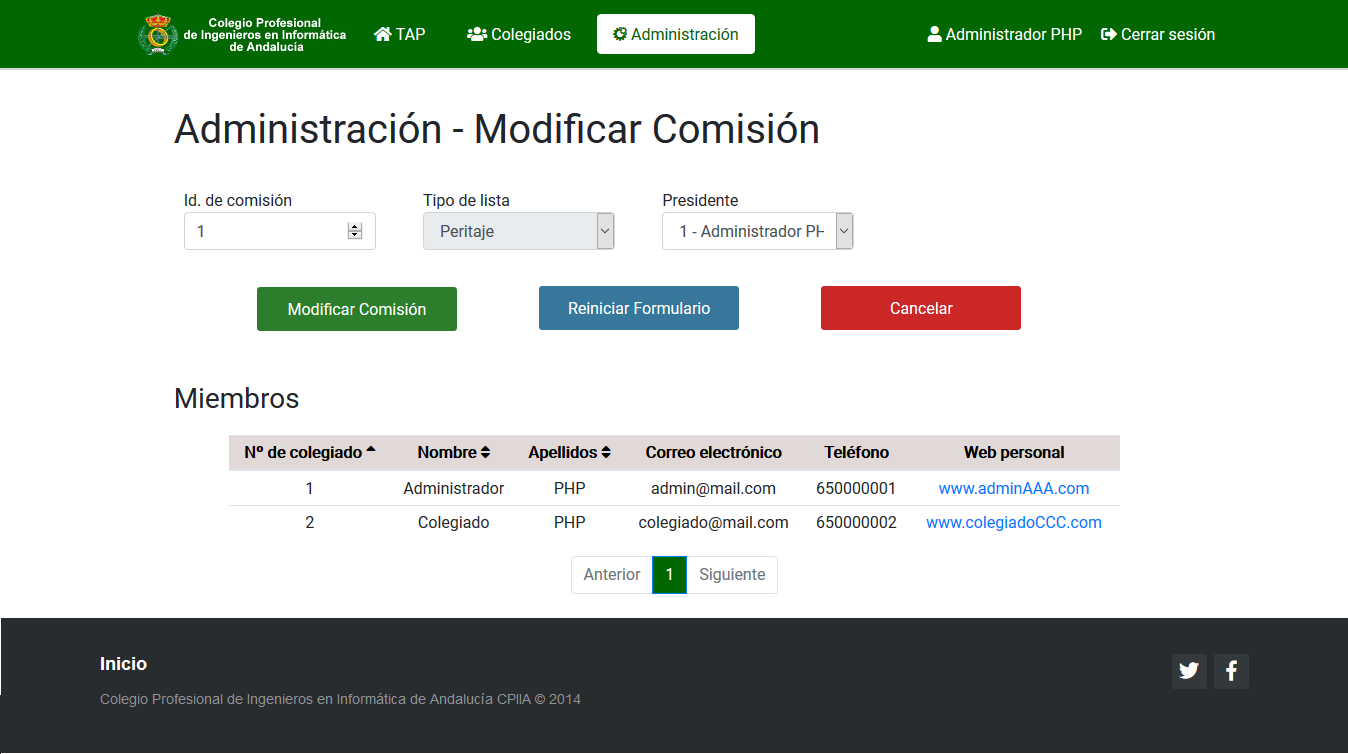
\includegraphics[width=150mm]{Web/Admin_ComisionModificar.png}
  \caption{Modificar Comisión}
  \label{fig:Web_Admin_ComisionModificar}
\end{figure}
\FloatBarrier

\addtocounter{figura_manual}{1} Por último, tenemos la ``Administración de Proyectos'' (\textbf{\hyperref[fig:Web_Admin_Proyectos]{Figura 6.\arabic{figura_manual}}}).\addtocounter{figura_manual}{1} Desde ella se puede acceder a la consulta (\textbf{\hyperref[fig:Web_Admin_ProyectoConsultar]{Figura 6.\arabic{figura_manual}}})\addtocounter{figura_manual}{1} o modificación (\textbf{\hyperref[fig:Web_Admin_ProyectoModificar]{Figura 6.\arabic{figura_manual}}}) de los proyectos ya existentes. A diferencia de las otras vistas de administración, en esta no se puede crear proyectos, ya que esta función se realiza durante las solicitudes de actuación (\textbf{\hyperref[fig:Web_TAP_SolicitarActuacion]{Figura 6.2}}). 

\begin{figure}[!htbp]
  \centering
  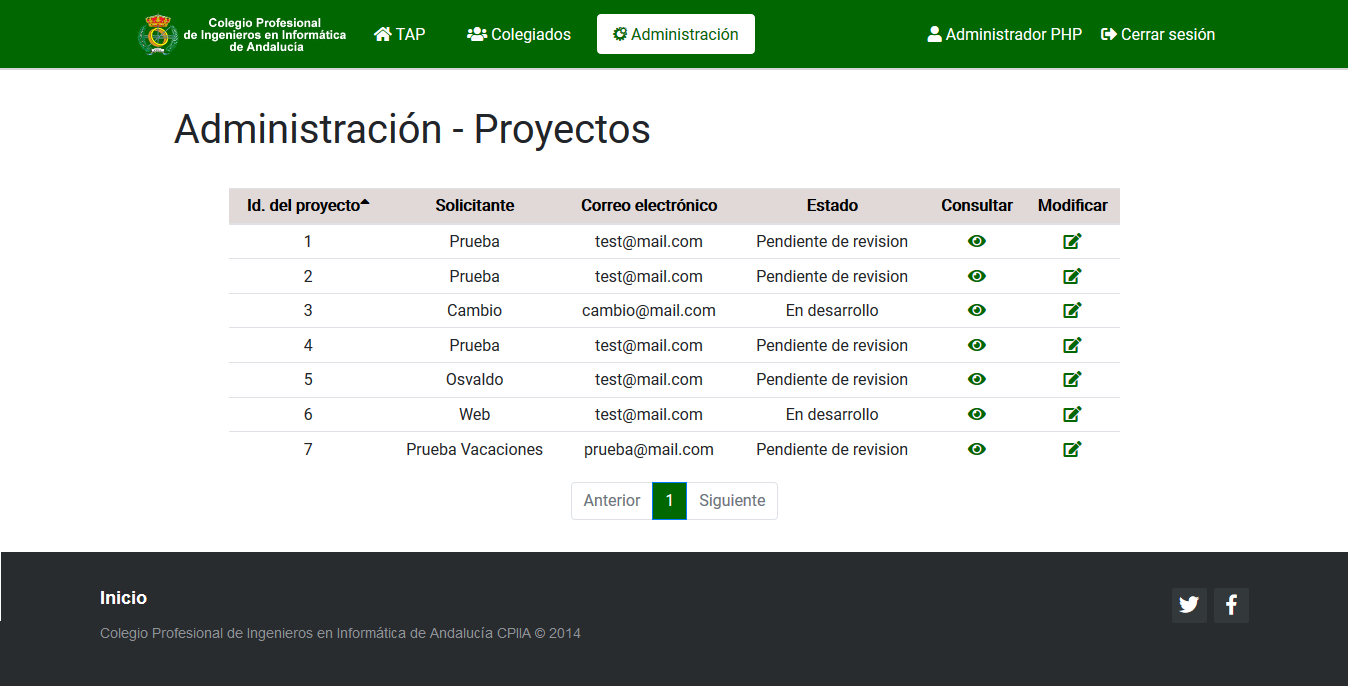
\includegraphics[width=150mm]{Web/Admin_Proyectos.png}
  \caption{Administración de Proyectos}
  \label{fig:Web_Admin_Proyectos}
\end{figure}
\FloatBarrier

\begin{figure}[!h]
  \centering
  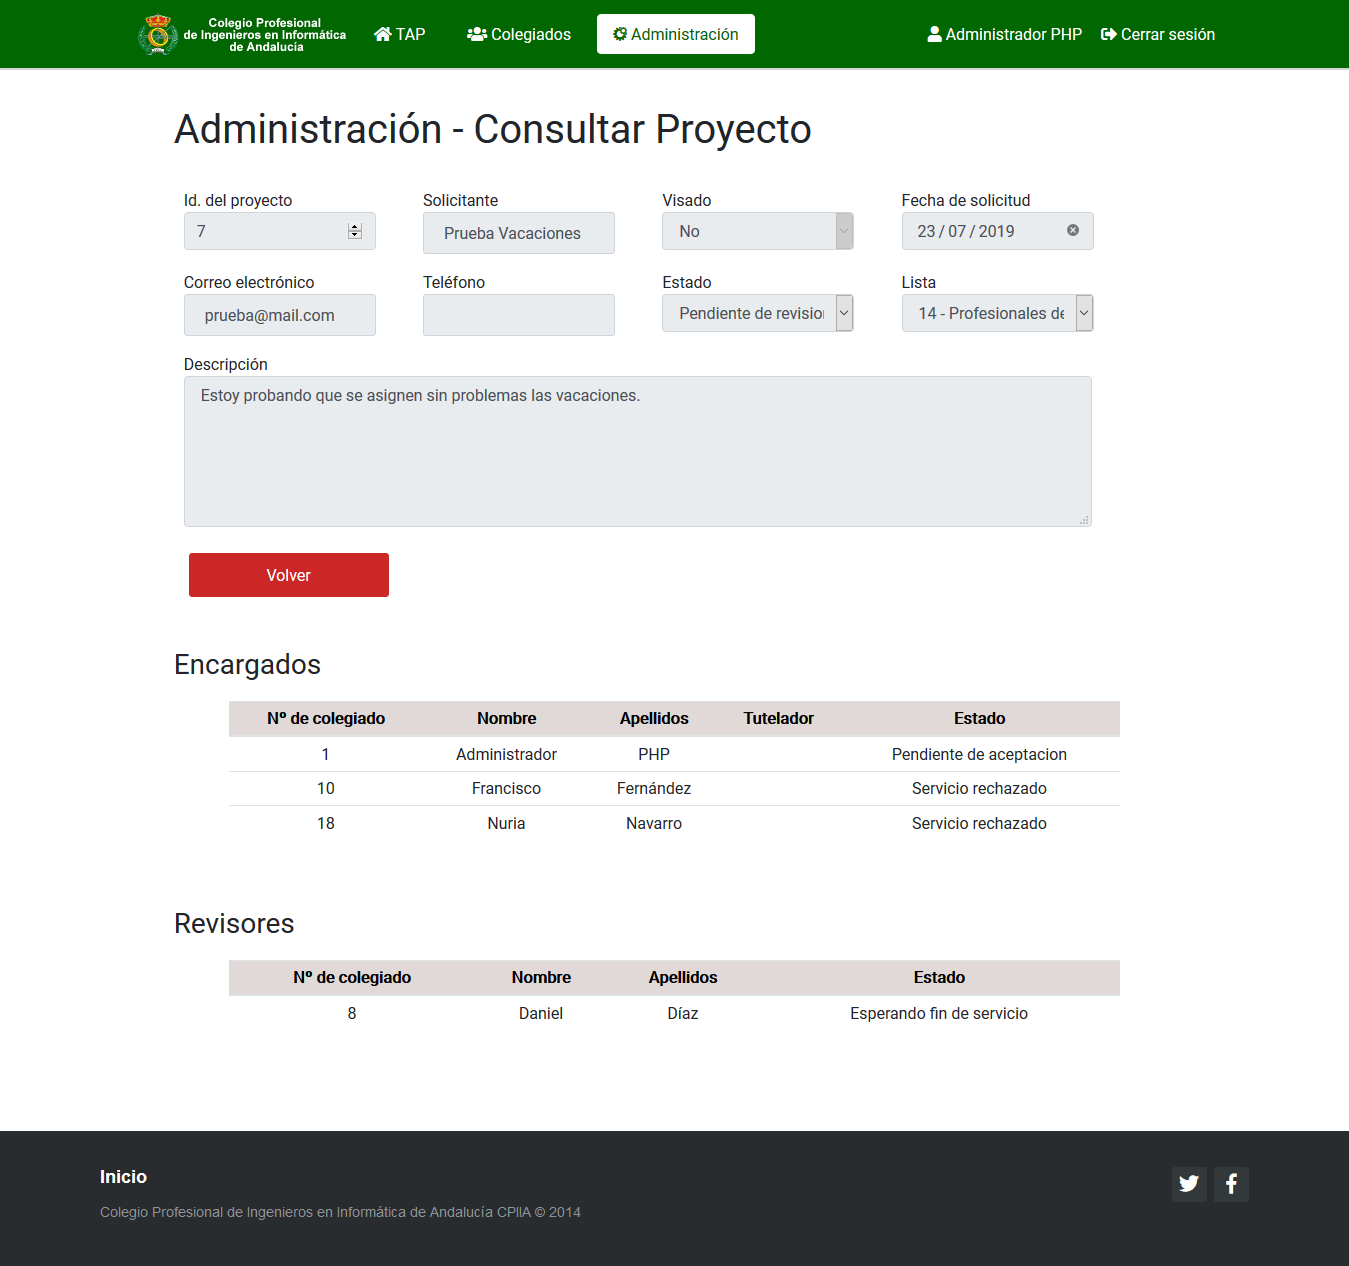
\includegraphics[width=150mm]{Web/Admin_ProyectoConsultar.png}
  \caption{Consultar Proyecto}
  \label{fig:Web_Admin_ProyectoConsultar}
\end{figure}
\FloatBarrier

Desde ``Modificar Proyecto'' (\textbf{\hyperref[fig:Web_Admin_ProyectoModificar]{Figura 6.\arabic{figura_manual}}}),\addtocounter{figura_manual}{1} también es posible acceder a la vista de ``Actualizar Estado de Visado'' (\textbf{\hyperref[fig:Web_Admin_ProyectoActualizarVisado]{Figura 6.\arabic{figura_manual}}}).
\begin{figure}[!h]
  \centering
  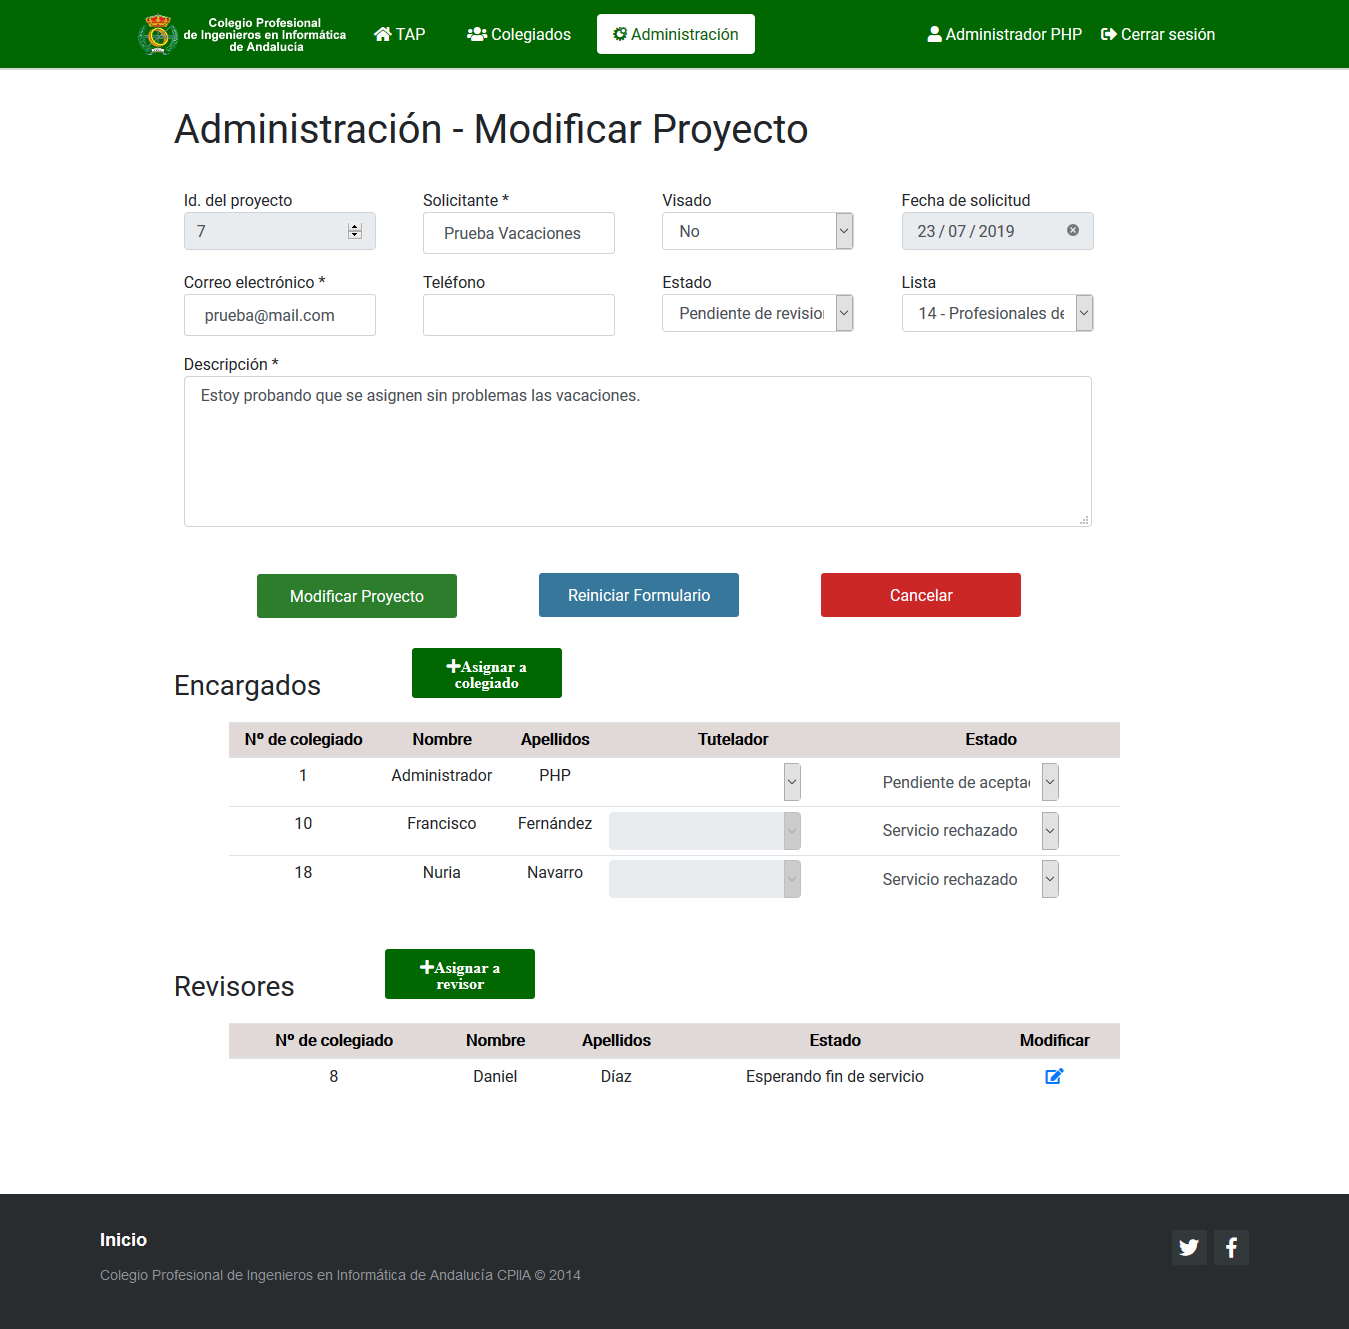
\includegraphics[width=150mm]{Web/Admin_ProyectoModificar.png}
  \caption{Modificar Proyecto}
  \label{fig:Web_Admin_ProyectoModificar}
\end{figure}
\FloatBarrier

\begin{figure}[!h]
  \centering
  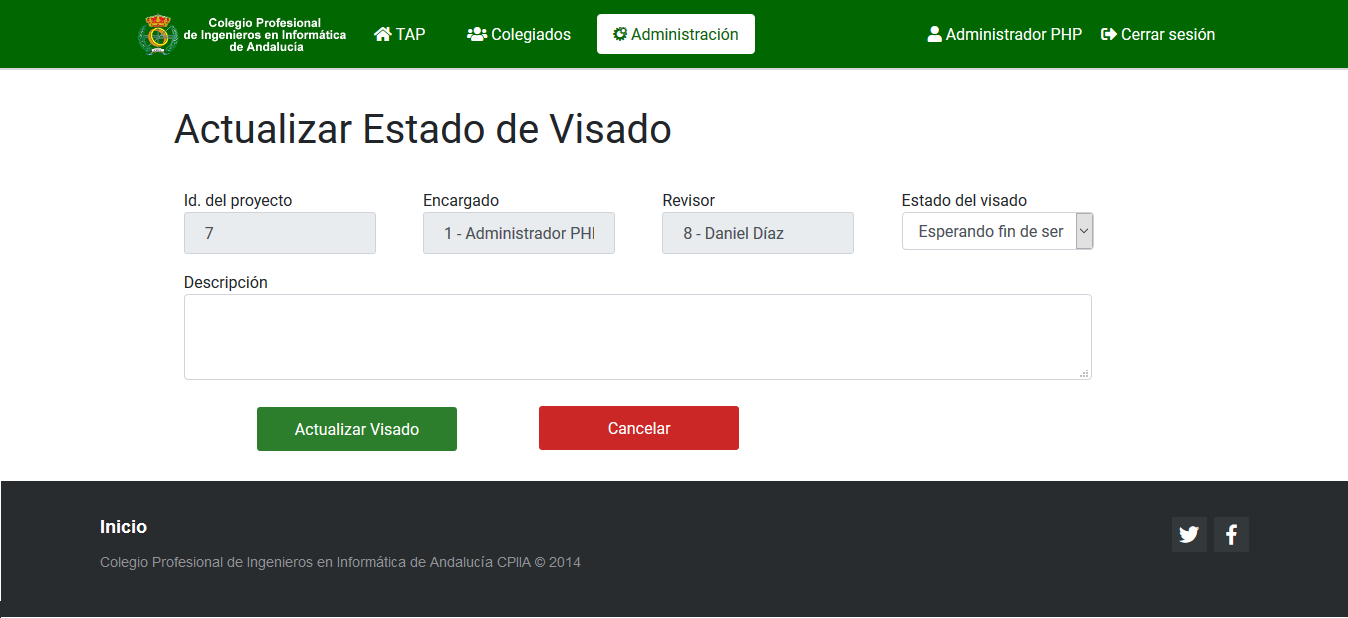
\includegraphics[width=150mm]{Web/Admin_ProyectoActualizarVisado.png}
  \caption{Actualizar Estado de Visado}
  \label{fig:Web_Admin_ProyectoActualizarVisado}
\end{figure}
\FloatBarrier